
% ============================================================
%  SECTION 1 : CLASSE DU DOCUMENT ET OPTIONS GLOBALES
% ============================================================

\documentclass[
12pt,          % Taille de police (10pt, 11pt, 12pt)
a4paper,       % Format du papier
oneside,      % Supprime les pages vierges entre chapitres
openright      % Les chapitres commencent toujours à droite
]{report}          % "report" = pour mémoires/thèses (chapitres numérotés)


% ============================================================
%  SECTION 2 : ENCODAGE ET LANGUE
% ============================================================

\usepackage[authoryear, round]{natbib}
\usepackage[utf8]{inputenc}       % Accepte les caractères accentués (é, à, ç...)
\usepackage[T1]{fontenc}          % Encodage des polices de sortie
\usepackage[french]{babel}        % Typographie française (guillemets, etc.)
% --> Remplacer "french" par "english" si besoin


% ============================================================
%  SECTION 3 : POLICES ET TYPOGRAPHIE
% ============================================================

\usepackage{palatino}             % Police Palatino (élégante, académique)
\usepackage{microtype}            % Optimise l'espacement des caractères
% (crénage, justification parfaite)



% ============================================================
%  SECTION 4 : MISE EN PAGE
% ============================================================

\usepackage[
top=2.5cm,          % Marge supérieure
bottom=2.5cm,       % Marge inférieure
left=3cm,           % Marge gauche (plus grande pour reliure)
right=2.5cm,        % Marge droite
headheight=15pt     % Hauteur de l'en-tête
]{geometry}

\usepackage{setspace}
\onehalfspacing               % Interligne 1.5 (standard académique)
% Alternatives : \singlespacing, \doublespacing

\setlength{\parskip}{6pt}     % Espace entre paragraphes
\setlength{\parindent}{1.5em} % Indentation du premier alinéa


% ============================================================
%  SECTION 5 : COULEURS (PERSONNALISEZ ICI VOS COULEURS)
% ============================================================

\usepackage[dvipsnames, table]{xcolor}

% --- Définir vos propres couleurs ---
% Conseil : choisissez 2-3 couleurs cohérentes avec votre institution
\definecolor{couleurPrimaire}{RGB}{0, 71, 130}    % Bleu institutionnel
\definecolor{couleurblack}{RGB}{0, 0, 0}  % Noir
\definecolor{couleurFond}{RGB}{245, 248, 252}      % Fond très léger
\definecolor{couleurSecondaire}{RGB}{198,40,40}
\definecolor{couleurTertiaire}{RGB}{27,120,80}
\definecolor{couleurGris}{RGB}{100,100,100}
\definecolor{couleurOr}{RGB}{180,130,20}


% ============================================================
%  SECTION 6 : EN-TÊTES ET PIEDS DE PAGE
% ============================================================

\usepackage{fancyhdr}
\pagestyle{fancy}

\fancyhf{}  % Effacer le style par défaut

% --- En-tête ---
\fancyhead[LE,RO]{                              % Gauche pages paires, Droite pages impaires
	\small\textcolor{couleurGris}{\leftmark}    % Nom du chapitre courant
}
\fancyhead[LO,RE]{                              % Droite pages paires, Gauche pages impaires
	\small\textcolor{couleurGris}{              % <-- REMPLACER PAR VOTRE TITRE COURT
		%Rapport sur la satisfaction des étudiants par rapport aux services universitaires.
	}
}

% --- Pied de page ---
\fancyfoot[C]{
	\textcolor{couleurGris}{\thepage}           % Numéro de page centré
}




% ============================================================
%  SECTION 7 : STYLE DES CHAPITRES ET TITRES (EFFET VISUEL)
% ============================================================


\usepackage{titlesec}
\usepackage{xcolor}
\titleformat{\chapter}
{\normalfont\Large\bfseries\color{black}}{\thechapter}{1em}{}
\titleformat{\section}
{\normalfont\large\bfseries\color{black}}{\thesection}{1em}{}
\titleformat{\subsection}
{\normalfont\normalsize\bfseries\color{black}}{\thesubsection}{1em}{}
\titleformat{\subsubsection}
{\normalfont\normalsize\bfseries\color{black}}{\thesubsubsection}{1em}{}
\usepackage{titletoc}

% --- Style des CHAPITRES ---
% Ce bloc crée un bandeau coloré en haut de chaque chapitre
\titleformat{\chapter}[display]
{\normalfont\bfseries\color{white}}         % Police du titre
{%
	\colorbox{couleurPrimaire}{%            % Bandeau de fond coloré
		\parbox{\dimexpr\textwidth+2\fboxsep\relax}{%
			\vspace{6pt}
			\hspace{10pt}
			\Large\color{white}
			\chaptertitlename~\thechapter   % Affiche "Chapitre 1"
			\vspace{6pt}
		}%
	}%
}
{0pt}
{%
	\colorbox{couleurSecondaire!20}{%       % Fond clair pour le nom du chapitre
		\parbox{\dimexpr\textwidth+2\fboxsep\relax}{%
			\vspace{8pt}
			\hspace{10pt}
			\huge
			\vspace{8pt}
		}%
	}%
	\vspace{-\baselineskip}
	\huge\color{couleurPrimaire}
}
[\vspace{10pt}\color{couleurPrimaire}\hrule\vspace{20pt}]

%

% --- Style des SECTIONS ---
\titleformat{\section}
{\normalfont\Large\bfseries\color{couleurPrimaire}}
{\thesection}{1em}{}
[\vspace{2pt}{\color{couleurPrimaire!40}\titlerule[0.5pt]}]

% --- Style des SOUS-SECTIONS ---
\titleformat{\subsection}
{\normalfont\large\bfseries\color{couleurblack}}
{\thesubsection}{1em}{}

% --- Style des SOUS-SOUS-SECTIONS ---
\titleformat{\subsubsection}
{\normalfont\normalsize\bfseries\color{couleurblack}}
{\thesubsubsection}{1em}{}

% --- Espacement autour des titres ---
\titlespacing*{\chapter}{0pt}{0pt}{30pt}
\titlespacing*{\section}{0pt}{20pt}{8pt}
\titlespacing*{\subsection}{0pt}{15pt}{6pt}
\titlespacing*{\subsubsection}{0pt}{10pt}{4pt}


% ============================================================
%  SECTION 8 : TABLEAUX ET FIGURES
% ============================================================
\usepackage{array}             % Options avancées des colonnes
\usepackage{booktabs}          % Tableaux professionnels (\toprule etc.)
\usepackage{tabularx}          % Tableaux à largeur ajustable
\usepackage{graphicx}          % Inclure des images
\usepackage{float}             % Option [H] pour forcer la position
\usepackage{multirow}          % Fusionner des cellules (lignes)
\usepackage{multicol}          % Fusionner des cellules (colonnes)
\usepackage{caption}           % Personnaliser les légendes
\usepackage{subcaption}        % Sous-figures côte à côte
\usepackage{longtable}         % Tableaux sur plusieurs pages


% --- Style des légendes (Figure 1, Tableau 1) ---
\captionsetup{
	font=small,
	labelfont={bf, color=couleurPrimaire},
	labelsep=period,
	skip=2pt
}
% Réduction des espaces autour des figures
\setlength{\textfloatsep}{3pt plus 1pt minus 1pt}
\setlength{\intextsep}{3pt plus 1pt minus 1pt}
\setlength{\abovecaptionskip}{2pt}
\setlength{\belowcaptionskip}{0pt}
\setlength{\floatsep}{4pt}

% --- Style des lignes de tableaux alternées ---
\newcommand{\rowcoleur}{\rowcolor{couleurFond}}


% ============================================================
%  SECTION 9 : MATHÉMATIQUES
% ============================================================

\usepackage{amsmath}           % Équations avancées (align, equation*, etc.)
\usepackage{amssymb}           % Symboles mathématiques (\mathbb, \nabla...)
\usepackage{amsthm}            % Théorèmes, définitions, preuves
\usepackage{mathtools}         % Compléments amsmath


% ============================================================
%  SECTION 10 : BOÎTES D'INFORMATION (ENCADRÉS STYLISÉS)
% ============================================================

\usepackage{tcolorbox}
\tcbuselibrary{skins, breakable, theorems}

% --- Boîte "Information" bleue ---
\newtcolorbox{boiteInfo}[1][Information]{
	enhanced,
	colback=couleurPrimaire!8,
	colframe=couleurPrimaire,
	boxrule=0.5pt,
	leftrule=4pt,
	arc=2pt,
	fonttitle=\bfseries\small\color{white},
	title=#1,
	attach boxed title to top left={yshift=-2mm, xshift=5mm},
	boxed title style={colback=couleurPrimaire, arc=1pt},
	breakable
}

% --- Boîte "Attention" rouge ---
\newtcolorbox{boiteAlerte}[1][Attention]{
	enhanced,
	colback=couleurSecondaire!8,
	colframe=couleurSecondaire,
	boxrule=0.5pt,
	leftrule=4pt,
	arc=2pt,
	fonttitle=\bfseries\small,
	title=#1,
	coltitle=couleurSecondaire,
	breakable
}

% --- Boîte "Résultat clé" verte ---
\newtcolorbox{boiteResultat}[1][Résultat clé]{
	enhanced,
	colback=couleurTertiaire!8,
	colframe=couleurTertiaire,
	boxrule=0.5pt,
	leftrule=4pt,
	arc=2pt,
	fonttitle=\bfseries\small,
	title=#1,
	coltitle=couleurTertiaire,
	breakable
}


% ============================================================
%  SECTION 11 : LIENS HYPERTEXTE ET RÉFÉRENCES
% ============================================================

\usepackage[
colorlinks=true,
linkcolor=couleurPrimaire,      % Liens internes (sections, figures)
citecolor=couleurTertiaire,     % Liens bibliographiques
urlcolor=couleurSecondaire,     % Liens URL
filecolor=couleurGris,
%pdftitle={Rapport sur la satisfaction des étudiants de l'Université NAZI BONI par rapport aux services universitaires },  % <-- MODIFIER
pdfauthor={SAKO Biton F.B.Cherif \\ ILIBOUDO B.G Bryand \\ BAYARA Orianne},                              % <-- MODIFIER
pdfsubject={Rapport de projet},
pdfkeywords={Satisfaction des étudiants de l'Université NAZI BONI}
]{hyperref}


% ============================================================
%  SECTION 12 : BIBLIOGRAPHIE
% ============================================================


% \usepackage[backend=biber,style=authoryear]{biblatex}
%\addbibresource{references.bib}


% ============================================================
%  SECTION 13 : PACKAGES DIVERS UTILES
% ============================================================

\usepackage{enumitem}             % Personnaliser les listes
\usepackage{pifont}               % Symboles spéciaux (coche, croix...)
% \usepackage{fontawesome5}       % Icônes (désactivé si non installé)
\usepackage{csquotes}             % Guillemets typographiques corrects
\usepackage{lipsum}               % Texte de remplissage (à supprimer)
\usepackage{pdflscape}            % Pages en paysage (\begin{landscape})
	\usepackage{rotating}             % Rotation de tableaux/figures
	\usepackage{afterpage}            % Insérer du contenu après la page
	
	
	% ============================================================
	%  SECTION 14 : COMMANDES PERSONNALISÉES (RACCOURCIS)
	% ============================================================
	
	% Commande pour mettre en avant un terme important
	\newcommand{\terme}[1]{\textbf{\textcolor{couleurPrimaire}{#1}}}
	
	% Commande pour une note marginale stylisée
	\newcommand{\noteImportante}[1]{%
		\begin{boiteAlerte}[Note importante]#1\end{boiteAlerte}%
	}
	
	% Commande pour les abréviations
	\newcommand{\abrev}[2]{\textbf{#1} (#2)}
	% Utilisation : \abrev{OMS}{Organisation Mondiale de la Santé}
	
	% Commande : IRR en gras
	\newcommand{\IRR}[1]{\textbf{IRR = #1}}
	
	
	% ============================================================
	%  SECTION 15 : NUMÉROTATION ET TABLE DES MATIÈRES
	% ============================================================
	
	\setcounter{tocdepth}{3}        % Profondeur de la TDM (jusqu'aux subsubsection)
	\setcounter{secnumdepth}{3}     % Numéroter jusqu'aux subsubsection
	
	
	% ============================================================
	%  ###  DÉBUT DU DOCUMENT  ###
	% ============================================================
	
	\begin{document}
		
		\pagenumbering{roman}   % Pages préliminaires numérotées en romain (i, ii, iii...)
		
		
		% ============================================================
		%  PAGE DE GARDE (PAGE 1)
		% ============================================================
		% Pour recréer une page de garde similaire au rapport original,
		% nous n'utilisons pas \maketitle mais une page personnalisée.
		
		\begin{titlepage}
			\thispagestyle{empty}
			
			% ── Cadre bleu autour de toute la page de garde ──
			\begin{tcolorbox}[
				enhanced,
				colback=white,
				colframe=couleurPrimaire,
				boxrule=2.5pt,
				arc=0pt,
				left=10pt, right=10pt,
				top=8pt, bottom=8pt,
				height=\dimexpr\textheight-2pt\relax,
				valign=top
			]
			
			\noindent
			\begin{minipage}[t]{0.48\textwidth}
				\centering
				{\footnotesize\textsc{MINISTÈRE DE L'ENSEIGNEMENT
						SUPÉRIEUR\\DE LA RECHERCHE ET DE L'INNOVATION}}\\[2pt]
				\textcolor{couleurPrimaire}{* * * * * * * * * * * *}\\[8pt]
				
\includegraphics[width=2.5cm]{logo_bf.png}
			\end{minipage}
			\hfill
			\begin{minipage}[t]{0.48\textwidth}
				\centering
				{\footnotesize\textsc{UNIVERSITÉ NAZI BONI}}\\[2pt]
				\textcolor{couleurPrimaire}{* * * * * * * * * * * *}\\[2pt]
				{\footnotesize\textsc{UNITÉ DE FORMATION ET DE\\
						RECHERCHE EN SCIENCES EXACTES\\
						ET APPLIQUÉES}}\\[2pt]
				\textcolor{couleurPrimaire}{* * * * * * * * * * * *}\\[2pt]
				{\footnotesize\textsc{LICENCE EN STATISTIQUES ET
						INFORMATIQUE}}\\[8pt]
				
\includegraphics[width=2.5cm]{logo_unb.png}
			\end{minipage}
			
			\vspace{0.8cm}
			
			\begin{center}
				{\Large\textbf{\textcolor{couleurPrimaire}{RAPPORT DE PROJET}}}\\[5pt]
				{\small\textit{Sur le thème :}}
			\end{center}
			
			\vspace{0.3cm}
			\begin{tcolorbox}[
				enhanced,
				colback=couleurPrimaire!8,
				colframe=couleurPrimaire,
				boxrule=1pt,
				arc=6pt,
				halign=center,
				left=8pt, right=8pt,
				top=6pt, bottom=6pt
				]
				\begin{center}
					\large\bfseries\color{black}
					Analyse sur la satisfaction des \'etudiants\\
					de l'universit\'e NAZI BONI\\
					par rapport aux services universitaires.
				\end{center}
			\end{tcolorbox}
			
			\vspace{0.5cm}
			\begin{center}
				{\small\textit{Présenté par :}}\\[5pt]
				{\Large\bfseries\color{couleurPrimaire}
					BAYARA Orianne.E.A\\
					ILBOUDO B.G.Bryan\\
					SAKO Biton F.B. Cherif
				}
			\end{center}
			
			\vspace{0.5cm}
			
			\noindent
			\begin{minipage}[t]{0.48\textwidth}
				\underline{\small\textbf{Charg\'e du cours :}}\\[4pt]
				TRAORE Issouf
			\end{minipage}
			
			\vfill
			\begin{center}
				\small
				\textbf{Période du projet :} Du 08 Février 2026 au 09 Mars 2026
				\hfill
				\textbf{Année académique :} 2025--2026
			\end{center}
			
			\end{tcolorbox}
		\end{titlepage}
		\clearpage
		% --- TABLE DES MATIÈRES (titre supprimé) ---
		{\renewcommand{\contentsname}{Table des matieres}
			\tableofcontents}
		\vspace{-2cm}
		\pagenumbering{arabic}
		\setcounter{page}{1}
		
		% --- RÉSUMÉ (texte libre, sans boîte) ---
		\chapter*{R\'ESUM\'E}
		\addcontentsline{toc}{chapter}{R\'ESUM\'E}
		\markboth{R\'ESUM\'E}{R\'ESUM\'E}
		
		La satisfaction des \'etudiants constitue un indicateur incontournable de la qualit\'e
		des services offerts par les institutions d'enseignement sup\'erieur. Dans un
		contexte o\`u les universit\'es africaines font face \`a des d\'efis croissants
		en mati\`ere de services administratifs, d'encadrement p\'edagogique et des services sociaux, d'infrastructure, \'evaluer le niveau de satisfaction des étudiants s'impose comme une n\'ecessit\'e
		pour toute d\'emarche d'am\'elioration continue.
		La pr\'esente \'etude analyse la satisfaction des \'etudiants de l'Universit\'e
		Nazi Boni (UNB) de Bobo-Dioulasso vis-\`a-vis des services universitaires.
		Elle s'appuie sur une enqu\^ete transversale men\'ee par les \'etudiants de troisi\'eme ann\'ee de
		LSI en 2024 dans le but d'\'evaluer la satisfaction des \'etudiants par rapport aux services universitaires de l'Universit\'e Nazi BONI. Le n\'ettoyage ainsi que l'analyse statistique de la base brute ont été m\'en\'es à l'aide du logiciel  STATA 14. 
		L'analyse de la base a \'et\'e m\'en\'ee sur 929 \'etudiants dont 350 femmes et 562 hommes avec 17 \'etudiants qui ont pr\'er\'efé garder l'anonymat par rapport à leur sexe. Avec un \^age moyen de 22,39 ans, les \'etudiants se r\'epartissent de façon in\'egale selon les caract\`eres
		sociod\'emographiques.
		Les r\'esultats indiquent un niveau de satisfaction globale variant selon le genre et les \'ecoles de formation.
		 Les services les mieux \'evalu\'es	sont \textbf{L'expérimentation des enseignants et la diversités des filières proposées par l'UNB} tandis que les plus
		critiqu\'es concernent \textbf{L'adaptation des étudiants handicapés et l'\'efficacit\'e des transports}. Des disparit\'es significatives sont observ\'ees
		selon la fili\`ere ($p < 0.05$) et le niveau d'\'etudes.
		Ces r\'esultats invitent l'administration de l'UNB \`a prioriser
		des investissements cibl\'es dans les domaines les moins satisfaisants,
		en associant les \'etudiants aux d\'ecisions d'am\'elioration.
		
		\vspace{12pt}
		\noindent\textbf{Mots-clés :}
		\textit{Satisfaction \'etudiante, Services universitaires, Universit\'e Nazi Boni, Enseignement sup\'erieur.}
		
				\cleardoublepage
		
		% --- ABSTRACT ---
		\chapter*{ABSTRACT}
		\addcontentsline{toc}{chapter}{ABSTRACT}
		\markboth{ABSTRACT}{ABSTRACT}
		
			% <-- TRADUCTION ANGLAISE DE VOTRE RÉSUMÉ
		Student satisfaction is a key indicator of the quality
		of services provided by higher education institutions.
		In a context where African universities face growing
		challenges in administrative services, academic
		supervision, social services and infrastructure,
		assessing student satisfaction has become an essential
		requirement for any continuous improvement process.
		
		This study analyses the satisfaction of students at
		Universit\'e Nazi Boni (UNB) in Bobo-Dioulasso with
		regard to university services. It draws on a
		cross-sectional survey conducted in 2024 by third-year
		LSI students, aimed at evaluating student satisfaction
		with the university services offered at UNB. Data
		cleaning and statistical analysis of the raw dataset
		were carried out using \textbf{STATA~14}.
		
		The analysis was conducted on a sample of $929$
		students, comprising $350$ women, $562$ men, and $17$
		students who preferred to remain anonymous regarding
		their gender. With a mean age of $22.39$ years,
		students are unevenly distributed across
		sociodemographic characteristics.
		
		The results indicate that overall satisfaction varies
		according to gender and field of study. The
		best-evaluated services are \textbf{teaching staff
			experience} and \textbf{the diversity of programmes
			offered by UNB}, while the most criticised concern
		\textbf{the adaptation of services for students with
			disabilities} and \textbf{the effectiveness of
			transportation}. Significant disparities are observed
		according to field of study ($p < 0.05$) and academic
		level.
		
		These findings call on the UNB administration to
		prioritise targeted investments in the least
		satisfactory areas, while actively involving students
		in improvement decisions.
	
	\vspace{0.5cm}
	\noindent\textbf{Key words:} Student satisfaction,
	University services,Universit\'e 
	Nazi Boni, Higher education .
		
		\cleardoublepage
		
		
		% --- LISTE DES ABRÉVIATIONS ---
		\chapter*{LISTE DES ABR\'EVIATIONS}
		\addcontentsline{toc}{chapter}{LISTE DES ABR\'EVIATIONS}
		\markboth{LISTE DES ABR\'EVIATIONS}{LISTE DES ABR\'EVIATIONS}
		
		\begin{tabbing}
			\hspace{4cm} \= \kill   % Définit la largeur de la colonne gauche
			% <-- FORMAT : SIGLE \> Signification complète \\
			\textbf{UNB}  \> Université NAZI BONI \\[3pt]
			\textbf{UFR}    \> Unité de Formation et de Recherche \\[3pt]
			\textbf{RU}   \> Restaurant universitaire \\[3pt]
			\textbf{SEA}   \> Sciences Exactes et Appliquées  \\[3pt]
			\textbf{INSSA}   \> Institut Supérieur des Sciences de la Santé \\[3pt]
			\textbf{IUT}   \>  Institut Universitaire de Technologie \\[3pt]
			\textbf{LSI}   \>  Licence en Statistiques Informatique \\[3pt]
			\textbf{SHLAM}   \>  Science Humaine Lettre Art Média\\[3pt]
			\textbf{SJPEG}   \> Science Juridique, Politique, Economique et de Gestion \\[3pt]
			\textbf{SVT}   \>  Sciences de la Vie et de la Terre \\[3pt]
			\textbf{ESI}   \>  Ecole Supérieure de l'Informatique \\[3pt]
			\textbf{IDR}   \>  Institut de Développement Rural \\[3pt]
			\textbf{UBC}   \>  Université BABA COULIBALY \\[3pt]
			\textbf{ROC}   \>  Receiver Operating Characteristic \\[3pt]
			
			% <-- AJOUTER VOS ABRÉVIATIONS
		\end{tabbing}
		
		\cleardoublepage
		
		% --- LISTE DES TABLEAUX ---
		\listoftables
		\addcontentsline{toc}{chapter}{Liste des Tableaux}
		\cleardoublepage
		
		% --- LISTE DES FIGURES ---
		\listoffigures
		\addcontentsline{toc}{chapter}{Liste des Figures}
		\cleardoublepage
	
		
		% ============================================================
		%  PRÉAMBULE (PRÉSENTATION FILIÈRE + STRUCTURE D'ACCUEIL)
		% ============================================================
		
		\chapter*{PR\'EAMBULE}
		\addcontentsline{toc}{chapter}{PR\'EAMBULE}
		\markboth{PR\'EAMBULE}{PR\'EAMBULE}
		\section*{PR\'ESENTATION DE LA FILIERE}
		% <-- PRÉSENTER VOTRE FILIÈRE (historique, objectifs, débouchés)
		Créée en septembre 1995, l'Université Nazi Boni (UNB) (ex Université Polytechnique de Bobo-Dioulasso) est située à une quinzaine de kilomètres de Bobo Dioulasso, précisément dans le village de Nasso. C'est un établissement public à caractère scientifique, culturel et technique, chargé de l'enseignement supérieur et de la recherche
		scientifique. Elle compte plusieurs Unités de Formation et de Recherche (UFR) parmi lesquelles figure l'UFR Sciences Exactes et Appliquées (SEA) (UFR/SEA) qui regroupe deux filières dont la Licence en Statistique et Informatique (LSI) et la filière Mathématiques Physique Chimie et Informatique. Créée en 2011, cette filière (LSI) forme des
		professionnels en statistiques, informatique et économie de niveau licence ayant pour rôle d'aider	les cadres supérieurs des entreprises, des Organisations Non Gouvernementales (ONG) et le gouvernement dans les prises de décisions.
		Ce cursus LSI s'étale sur trois (03) années d'études, réparties en six semestres. À l'issue de sa
		formation, l'étudiant en LSI doit être capable de :
		 organiser la collecte de l'information (enquête) ;
		 construire et gérer un système d'information (Base de données) ;
		 concevoir et planifier un sondage ;
		 concevoir et gérer un site web ;
		participer à un projet de développement d'application ;
		analyser, résumer et segmenter les vastes ensembles de données ;
		décrire, traiter, synthétiser des données d'enquête ;
		 analyser, décomposer, désaisonnaliser et modéliser des séries chronologiques ;
		 estimer et tester les effets d'un ensemble de facteurs.
	
		\cleardoublepage
		
		% --- INTRODUCTION (texte libre, sans boîte) ---
		\chapter*{INTRODUCTION}
		\addcontentsline{toc}{chapter}{INTRODUCTION}
		\markboth{INTRODUCTION}{INTRODUCTION}
		% Saisissez l'introduction
			L'université est bien plus qu'un simple lieu de transmission des savoirs: elle constitue un
		espace de vie, de socialisation et de développement personnel pour des milliers d'étudiants.
		À ce titre, la qualité des services qu'elle offre, qu'ils soient administratifs, pédagogiques, sociaux ou matériels conditionne largement les conditions d'études et de ce fait les performances académiques des apprenants. Dans un contexte mondial marqué par une concurrence accrue entre les établissements d'enseignement supérieur et par des exigences croissantes d'efficacité et de redevabilité, la satisfaction des usagers est devenue un indicateur incontournable de la qualité institutionnelle.
		En Afrique subsaharienne, et particulièrement au Burkina Faso, les universités publiques font
		face à des défis structurels importants: surpopulation des amphithéâtres, insuffisance des
		infrastructures, précarité des ressources numériques et difficultés d'accès aux services
		sociaux de base. Dans ce contexte, l'Université Nazi Boni (UNB) de Bobo-Dioulasso ne fait
		pas exception. Fondée pour répondre aux besoins de formation de la région ouest du Burkina
		Faso, elle accueille des étudiants issus de divers établissements: l'ESI, l'INSSA, l'IDR,
		l'IUT, l'UFR-SEA, l'UFR-SVT, l'UFR-SHLAM et l'UFR-SJPEG. La diversité de ces structures,
		aux missions et aux réalités très différentes, rend d'autant plus nécessaire une évaluation
		systématique et rigoureuse de la satisfaction des étudiants.
		C'est dans cette perspective que s'inscrit la présente étude, conduite par les étudiants de
		troisième année de Licence en Statistique et Informatique (LSI) de l'UNB. À partir d'une
		enquête menée auprès d'un large échantillon d'étudiants, ce travail vise à mesurer et à
		expliquer les niveaux de satisfaction relatifs aux services administratifs, pédagogiques,
		sociaux ainsi qu'aux infrastructures et équipements. Les résultats obtenus permettront de
		formuler des recommandations concrètes à l'intention des autorités académiques et
		administratives, en vue d'une amélioration continue des services offerts.
		Le présent rapport est structuré comme suit: après avoir présenté le contexte et la
		justification de l'étude, nous formulerons la problématique et les objectifs de recherche.
		Nous procéderons ensuite à une revue de la littérature, avant d'exposer la méthodologie
		adoptée. Les résultats seront ensuite présentés et discutés, et le rapport s'achèvera par
		une conclusion assortie de recommandations.
		\vspace{12pt}
		\cleardoublepage
		
		% ============================================================
		%  CHAPITRE 1 : PRÉSENTATION DE L'ÉTUDE / GÉNÉRALITÉS
		% ============================================================
		
		\chapter{Présentation de l'étude}
		\label{chap:presentation}
		
			\section{Contexte général}
		L'enseignement supérieur au Burkina Faso a connu une expansion significative au cours des
		deux dernières décennies. La création de nouvelles universités, dont l'Université Nazi Boni
		de Bobo-Dioulasso en 1995, témoigne de la volonté des pouvoirs publics d'élargir l'accès
		à l'enseignement supérieur et de désengorger l'Université Joseph Ki-Zerbo de Ouagadougou.
		Toutefois, cette croissance des effectifs ne s'est pas toujours accompagnée d'une amélioration
		proportionnelle des conditions d'études et des services offerts aux étudiants.
		L'UNB, établissement public d'enseignement supérieur et de recherche, accueille aujourd'hui
		des milliers d'étudiants répartis au sein de plusieurs structures de formation à savoir: sciences exactes, sciences de la vie, sciences humaines et sociales,
		droit et sciences politiques, informatique et statistique, ou encore agriculture et
		ressources naturelles. Cette diversité institutionnelle, si elle constitue une richesse,
		soulève également des interrogations quant à l'homogénéité et à l'équité dans la distribution
		des services universitaires.
		
		\section{Justification}
		La satisfaction des étudiants vis-à-vis des services universitaires constitue un volet
		important dans la qualification des établissements d'enseignement supérieur. Elle influe
		directement sur la motivation, la persévérance et les résultats académiques des apprenants
		\citep{elliott2001} \citep{letcher2010}.
		 Par ailleurs, dans une logique de
		gouvernance participative, recueillir et analyser l'opinion des étudiants
		permet aux institutions d'identifier leurs forces et leurs faiblesses et d'orienter leurs
		politiques d'amélioration.
		Au Burkina Faso, les données sur la satisfaction des étudiants à l'UNB sont rares et rarement
		produites en continuité. Cette lacune informationnelle constitue un obstacle à la
		prise de décision éclairée par les responsables académiques. La présente enquête, initiée
		dans le cadre pédagogique du cours de Pratique d'enquête du programme LSI III, répond à ce
		besoin en produisant des données de qualité sur la satisfaction des étudiants à
		l'UNB.
		
		
		\section{Problématique }
		\label{sec:problematique}
		
		% <-- EXPOSER LE PROBLÈME SCIENTIFIQUE QUE VOUS TRAITEZ
		% Structure suggérée :
		% 1. Situation mondiale/continentale
		% 2. Situation au Burkina Faso
		% 3. Lacune dans les connaissances
		% 4. Intérêt de votre étude
		Les universités africaines sont confrontées à un paradoxe. En effet, d'une part, elles
		doivent contenir un nombre croissant d'étudiants dans un contexte de ressources budgétaires
		limitées, d'autre part, elles sont appelées à offrir des services de qualité suffisante
		pour garantir des conditions d'études acceptables et favoriser la réussite académique. Ce
		paradoxe se fait d'autant plus ressentir à l'UNB, où la diversité des établissements et des publics
		estudiants complique encore davantage l'évaluation et la gestion de la satisfaction.
		On observe en pratique que les étudiants expriment régulièrement, des mécontentements relatifs à la qualité de l'accueil administratif, à l'insuffisance des infrastructures, à la qualité de la connexion Internet, au fonctionnement des services sociaux (restauration, logement, santé) ou encore à la pertinence des formations proposées. Cependant, ces perceptions restent rarement exploitées dans une optique d'amélioration des services.
		Dans ce contexte, plusieurs questions se posent:
		
		\begin{itemize}
			\item Quel est le niveau global de satisfaction des étudiants de l'UNB par rapport aux
			services universitaires~?
			\item Existe-t-il des disparités de satisfaction selon le genre, le niveau d'étude,
			l'âge ou l'établissement?
			\item Quels sont les déterminants de l'insatisfaction globale?
			\item Quels services enregistrent le plus de mécontentement et méritent une attention
			prioritaire de la part des autorités?
		\end{itemize}
		
		Ces interrogations constituent le fil directeur de la présente étude, qui entend apporter
		des éléments de réponse fondés sur des données collectées directement auprès
		des étudiants de l'UNB.
		
		\section{Objectifs de l'étude}
		\label{sec:objectifs}
		
		\subsection{Objectif général}
		L'objectif général de cette étude est d'évaluer le niveau de satisfaction des étudiants
		de l'Université Nazi Boni par rapport aux services universitaires et d'en identifier les
		principaux déterminants.
		
		\subsection{Objectifs spécifiques}
		De manière spécifique, il s'agira de:
		\begin{enumerate}
			\item Décrire la répartition des étudiants enquêtés selon leurs caractéristiques
			socio-démographiques (sexe, âge, établissement, niveau d'étude);
			\item Évaluer le niveau de satisfaction des étudiants par rapport aux services
			administratifs (accueil, inscriptions, délivrance de documents, communication,
			sécurité);
			\item Évaluer le niveau de satisfaction des étudiants par rapport aux services
			pédagogiques (qualité de la formation, pertinence des filières, gestion des stages,
			traitement des réclamations, bibliothèque);
			\item Évaluer le niveau de satisfaction des étudiants par rapport aux services sociaux
			(logement, santé, restauration, activités sportives et culturelles);
			\item Évaluer le niveau de satisfaction des étudiants par rapport aux infrastructures
			et équipements (Internet, mobilier, équipements informatiques, immobilier);
			\item Identifier les déterminants socio-démographiques de l'insatisfaction globale à
			travers un modèle de régression logistique.
		\end{enumerate}
		
		
		
		\section{Revue de la littérature}
		\label{sec:revue}
		% <-- SYNTHÈSE DES TRAVAUX EXISTANTS
		% Structure recommandée :
		% 1. Contexte mondial de la dengue
		% 2. Études en Afrique
		% 3. Études au Burkina Faso
		% 4. Ce que votre étude apporte de nouveau
		\subsection{Définition et mesure de la satisfaction des étudiants}
		La satisfaction des étudiants est un concept multidimensionnel qui renvoie à l'évaluation
		relative que font les apprenants de leur expérience universitaire globale au regard de
		leurs attentes initiales \citep{oliver1980}.
		 Elle englobe plusieurs aspects à savoir
		la qualité de l'enseignement, la disponibilité et la compétence du personnel, la qualité
		des infrastructures, l'accessibilité des services sociaux et bien d'autres aspects 
		\citep{pascarella1991how}.
		Plusieurs instruments ont été développés pour mesurer cette satisfaction. L'échelle de
		Likert à cinq points allant de \og{}Très insatisfait\fg{} à \og{}Très satisfait\fg{}
		est l'outil le plus couramment utilisé dans les enquêtes de satisfaction dans l'enseignement
		supérieur \citep{hill1995measuring}. 
		Elle permet une quantification simple et comparative
		des appréciations, tout en favorisant une analyse statistique robuste.
		
		\subsection{Facteurs influençant la satisfaction des étudiants}
		La littérature internationale identifie plusieurs catégories de facteurs susceptibles
		d'influencer la satisfaction des étudiants:
		\paragraph{Facteurs pédagogiques:} La qualité de l'enseignement est l'un des déterminants
		majeur de la satisfaction globale. La compétence, la disponibilité et la
		pédagogie des enseignants, ainsi que la pertinence des programmes au regard des réalités
		du marché du travail, sont des facteurs récurrents dans la littérature
		\citep{aldridge1998, wiers2002student}.
		\paragraph{Facteurs infrastructurels:} L'état des locaux, la disponibilité des équipements
		informatiques et la qualité de la connexion Internet jouent un rôle croissant dans la
		satisfaction des étudiants, notamment dans un contexte de numérisation des activités
		pédagogiques 
		\citep{wilkins2013}.
		\paragraph{Facteurs administratifs:} La réactivité et la courtoisie du personnel
		administratif, la transparence des procédures et la fluidité des processus d'inscription
		constituent des aspects importantes de l'expérience étudiante \citep{elliott2002}.
		\paragraph{Facteurs sociaux:} Les conditions de logement, l'accès aux soins de santé,
		la qualité de la restauration universitaire et l'offre d'activités culturelles et sportives
		contribuent à la satisfaction globale des étudiants, en particulier pour ceux qui résident
		loin de leur famille
		\citep{amole2009}.
		
		
		\section{Modélisation statistique de la satisfaction}
		Sur le plan méthodologique, la régression logistique est l'outil le plus fréquemment
		mobilisé pour identifier les déterminants d'une variable dépendante binaire telle que
		la satisfaction ou l'insatisfaction 
		\citep{hosmer2013applied}. 
		Elle permet d'estimer,
		toutes choses égales par ailleurs, l'effet propre de chaque variable explicative sur
		la probabilité de l'événement étudié. Les odds ratios (rapports de cotes) issus de
		ce modèle constituent une mesure intuitive de l'ampleur et du sens des effets estimés.
		
		
		
		\chapter{MÉTHODOLOGIE ET LOGICIEL UTILISÉ}
		% -----------------------------------------------
		% MÉTHODOLOGIE ET LOGICIEL UTILISÉ
		% -----------------------------------------------
		\section{Méthodologie et logiciel utilisé}
		
		\subsection{Source et nature des données}
		
		Les données utilisées dans cette étude sont issues d'une enquête transversale conçue et
		menée par les étudiants de troisième année de LSI de l'UNB au cours de l'année académique
		2023-2024. L'enquête a été réalisée à l'aide d'un questionnaire structuré administré en
		face-à-face auprès d'étudiants de l'UNB appartenant à différents établissements~: ESI,
		INSSA, IDR, IUT, UFR-SEA, UFR-SVT, UFR-SHLAM et UFR-SJPEG. La collecte s'est effectuée
		sur plusieurs sites de l'université.
		
		\subsection{Instrument de collecte}
		
		Le questionnaire est organisé en six grandes sections~:
		
		\begin{enumerate}
			\item Les informations socio-démographiques de l'étudiant (sexe, âge, établissement,
			niveau d'étude, nationalité)~;
			\item La satisfaction par rapport aux services administratifs (accueil, inscriptions,
			délivrance de documents, communication, sécurité)~;
			\item La satisfaction par rapport aux services pédagogiques (filières, qualité de la
			formation, stages, réclamations, bibliothèque)~;
			\item La satisfaction par rapport aux services sociaux (logement, santé, restauration,
			activités sportives et culturelles)~;
			\item La satisfaction par rapport aux infrastructures et équipements (Internet, mobilier,
			informatique, immobilier)~;
			\item Un espace de commentaires libres.
		\end{enumerate}
		
		Pour chaque dimension de satisfaction, une question principale est posée sur une échelle
		de Likert à cinq niveaux (1~= Très insatisfait~; 5~= Très satisfait), suivie d'une série
		d'affirmations soumises à l'accord ou au désaccord de l'enquêté.
		
		\subsection{Nettoyage et préparation des données}
		
		La base de données brute a fait l'objet d'un nettoyage rigoureux avant toute
		analyse. Ce travail a consisté à : renommer et labelliser les variables conformément au
		questionnaire, recoder les variables catégorielles, créer de nouvelles variables dérivées,
		notamment les scores de satisfaction par section et le score global de satisfaction,
		et traiter les valeurs manquantes ou aberrantes.
		
		Plus précisément, le nettoyage s'est articulé en cinq étapes successives.
		
		\textbf{Suppression des variables inutiles:}
		Toutes les variables liées à la collecte (métadonnées du formulaire telles
		que les identifiants, horodatages et statuts de validation) ont été supprimées, ainsi
		que les notes intermédiaires (\texttt{note\_adm}, \texttt{note\_ped}, etc.).
		
		\textbf{Conversion en numérique:}
		Une liste de variables à exclure (celles naturellement en chaîne de caractères :
		\texttt{sexe}, \texttt{etb}, commentaires libres et autres variables textuelles)
		a été définie. Ensuite, une boucle parcourt toutes les autres variables pour les convertir
		en numérique à l'aide de la commande \texttt{destring}.
		
		\textbf{Labelisation des variables:}
		Toutes les variables ont reçu un label descriptif clair.
		
		\textbf{Gestion des valeurs manquantes et recodages:}
		Nous avons recodé les nationalités manquantes (\texttt{nat == .}) en une catégorie
		\og Inconnue \fg{}. Ensuite les scores d'échelle portant la valeur \texttt{8} ( correspondant
		à une réponse non-applicable dans le formulaire) ont été recodés à \texttt{0}.
		Par ailleurs, une variable \texttt{tranches\_age} a été créée à partir de \texttt{age}
		en découpant la distribution en intervalles de deux ans (17--18, 19--20, \ldots, 27--28).
		
		\textbf{Recodage des variables de réponse en variables binaires:}
		Il s'est agit pour nous, de définir et d'appliquer un programme à l'ensemble des variables de réponse.
		Il prend une variable de référence (score d'échelle) et recode automatiquement les six
		variables de réponse associées. La valeur \texttt{100} est attribuée si la modalité
		correspondante a été cochée (dans l'optique de rendre plus simple l'affichage en pourcentage), \texttt{0} dans le cas contraire, et la valeur manquante
		(\texttt{.}) lorsque la réponse de référence est absente. Ces variables recodées ont
		ensuite reçu le label \texttt{choix} (0 = \og Non \fg{}, 100 = \og Oui \fg{}).
		
		La variable dépendante du modèle de régression logistique(la satisfaction globale)
		a été construite comme suit: elle prend la valeur 1 (insatisfait) si le score global de
		satisfaction est inférieur ou égal à 45 et la valeur 0 (satisfait) dans le cas contraire.
		
		\subsection{Méthodes d'analyse}
		
			L'analyse des données a été conduite en deux étapes~:
			
			\paragraph{Analyse descriptive:} Des statistiques descriptives univariées (effectifs,
			fréquences, moyennes) ont été produites pour chaque dimension de satisfaction et pour
			chaque variable socio-démographique. Des représentations graphiques (diagrammes en barres)
			ont été utilisées pour visualiser la distribution des réponses et faciliter l'interprétation.
			
			
			\paragraph{Analyse explicative (Régression logistique):} La variable \textit{insatisfaction globale} étant une variable qualitative dichotomique (être insatisfait ou ne pas l'être), la régression la plus appropriée est la régression logistique binaire. Cette régression permet d'estimer la probabilité de survenue d'un phénomène en fonction des variables explicatives.
			
			La variable dépendante de l'étude prend la valeur 1 si l'individu est globalement insatisfait et 0 sinon. En considérant $Y$ comme la variable dépendante et $X_1, X_2, X_3, \ldots, X_k$ les variables explicatives (sexe, groupe d'âge, niveau d'étude, établissement de rattachement), le modèle s'écrit :
			
			\begin{equation}
				Y = \alpha_0 + \alpha_1 X_1 + \alpha_2 X_2 + \alpha_3 X_3 + \cdots + \alpha_k X_k
			\end{equation}
			
			\noindent avec $\alpha_0$ la constante du modèle~; $\alpha_i$, $i = 1, \ldots, k$, les coefficients du modèle et $k$ le nombre de variables explicatives.
			
			\[
			Y = \begin{cases}
				1 & \text{si l'individu } i \text{ est globalement insatisfait} \\
				0 & \text{sinon}
			\end{cases}
			\]
			
			La probabilité qu'un individu $i$ soit globalement insatisfait s'écrit :
			
			\begin{equation}
				P(Y_i = 1 \mid X_k) = \frac{e^{\left(\alpha_0 + \sum_{k=1}^{n} \alpha_k X_k\right)}}{1 + 	e^{\left(\alpha_0 + \sum_{k=1}^{n} \alpha_k X_k\right)}}
			\end{equation}
			
			La probabilité qu'un individu $i$ ne soit pas globalement insatisfait est :
			
			\begin{equation}
				P(Y_i = 0 \mid X_k) = 1 - \frac{e^{\left(\alpha_0 + \sum_{k=1}^{n} \alpha_k X_k\right)}}{1 + 	e^{\left(\alpha_0 + \sum_{k=1}^{n} \alpha_k X_k\right)}} = \frac{1}{1 + e^{\left(\alpha_0 + \sum_{k=1}^{n} \alpha_k X_k\right)}}
			\end{equation}
			
			La qualité du modèle a été évaluée à l'aide du pseudo $R^2$ de McFadden, du test de Hosmer-Lemeshow et de la courbe ROC (aire sous la courbe, AUC). Les résultats sont présentés sous forme d'odds ratios avec leur niveau de significativité. Nous chercherons ainsi à expliquer l'insatisfaction globale par le sexe, le groupe d'âge, le niveau d'étude et l'établissement de rattachement des répondants.
			
		\textbf{Outils statistiques}
		\paragraph{Le test de Kruskal-Wallis}
		
		Le test de Kruskal-Wallis est un test non param\'etrique
		utilis\'e pour comparer les distributions de $k$ groupes
		ind\'ependants.
		
		\medskip
		\noindent Les hypoth\`eses du test sont~:
		\begin{itemize}
			\item $H_0$~: les $k$ groupes ont la m\^eme
			distribution (m\'edianes \'egales)
			\item $H_1$~: au moins un groupe diff\`ere
			significativement des autres
		\end{itemize}
		
		\medskip
		\noindent La statistique de test est~:
		\begin{equation}
			H = \frac{12}{N(N+1)}
			\sum_{i=1}^{k} \frac{R_i^2}{n_i}
			- 3(N+1)
		\end{equation}
		
		\medskip
		\noindent Sous $H_0$, la statistique $H$ suit
		approximativement une loi du $\chi^2$ \`a $k-1$
		degr\'es de libert\'e. On rejette $H_0$ si~:
		
		\begin{equation}
			H > \chi^2_{\alpha,\, k-1}
		\end{equation}
		
		
		\paragraph{Le test post-hoc de Mann-Whitney}
		Lorsque le test de Kruskal-Wallis conclut \`a une
		diff\'erence significative, des comparaisons par paires
		sont effectu\'ees \`a l'aide du test de Mann-Whitney,
		avec correction de Bonferroni pour contr\^oler le
		risque d'erreur de type~I li\'e aux comparaisons
		multiples.
		
		\medskip
		\noindent Pour deux groupes $i$ et $j$ d'effectifs
		$n_i$ et $n_j$, la statistique de Mann-Whitney est~:
		
		\begin{equation}
			U = n_i n_j +
			\frac{n_i(n_i + 1)}{2} - R_i
		\end{equation}
		
		
		\medskip
		\noindent Pour des grands \'echantillons, la statistique
		standardis\'ee est~:
		
		\begin{equation}
			Z = \frac{U - \mu_U}{\sigma_U}
		\end{equation}
		
		\noindent avec~:
		\begin{align}
			\mu_U    &= \frac{n_i n_j}{2} \\[6pt]
			\sigma_U &= \sqrt{\frac{n_i n_j (n_i + n_j + 1)}{12}}
		\end{align}
		
		\medskip
		\noindent La correction de Bonferroni ajuste le seuil
		de significativit\'e~: pour $m$ comparaisons
		simultan\'ees, le seuil retenu est~:
		
		\begin{equation}
			\alpha^* = \frac{\alpha}{m}
		\end{equation}
		
		\noindent Dans notre cas, avec $\alpha = 0{,}05$ et
		$m$ paires compar\'ees, toute paire dont la p-value
		est inf\'erieure \`a $\alpha^*$ est consid\'er\'ee
		comme significativement diff\'erente.
		
		
		\subsection{Logiciel utilisé}
		
		L'ensemble du nettoyage et des analyses statistiques a été réalisé avec le logiciel
		\textbf{Stata} (StataCorp, version~14). Stata a été retenu pour ses capacités robustes
		en analyse de données d'enquête, la richesse de ses commandes de régression logistique
		(\texttt{logit}, \texttt{logistic}) et la facilité d'exportation des résultats en
		format \textbf{LATEX} via la commande \texttt{outreg2} ou \texttt{esttab}. La rédaction du
		rapport a été effectuée avec \textbf{LATEX} sous \textbf{TeXstudio}, conformément aux
		instructions du projet.
	
		
		% ============================================================
		%  CHAPITRE 3 : RÉSULTATS ET DISCUSSION
		% ============================================================
		
		\chapter{Présentation des résultats	de l’étude}
		\label{chap:resultats}
		
		% <-- INTRO DU CHAPITRE
		Le but de ce chapitre est d’exposer les résultats de notre étude. Les résultats des différentes analyses seront exposés dans le dessein de parvenir à l’objectif générale de notre étude d’une part et à ses objectifs spécifiques d’autre part.
		
		
		\section{La répartition des étudiants enquêtés en fonction des catégories
			sociodémographiques}
		\label{sec:Analyse socio-démographique}
		
	Cette étude sur la satisfaction des étudiants par rapport aux services universitaires a été mené sur \textbf{929} étudiants. Ils se répartissent comme suite inégalement selon les catégories sociodémographiques telles le genre, la nationalité, l'âge, l'établissement et le niveau d'étude de l'étudiant. 
	Les étudiants enquêtés se composent de \textbf{350} femmes ( $38{,}4\%$) et \textbf{562} hommes ( $61{,}6\%$) sur \textbf{912} qui ont donné leur sexe et \textbf{17} autres qui ont gardé l'anonymat sur cet aspect.
    $98{,}9\%$ des enquêtés sont des \textbf{burkinabè}, les autres nationalités et les données manquantes représentent ensemble moins de $2\%$.
	L’âge minimum des enquêtés est 17 ans et le maximum est 28 ans, avec un intervalle interquartile [21-24].
	Selon les écoles de formation, environ un tiers de
	l’échantillon est constitué d’étudiants de l’IUT (28,8\%). L’UFR-SVT, l’IDR et le SEA comptent respectivement 17,2\%, 10,2\% et 15,9\%. Les établissements SHLAM, SJPEG et INSSA sont moins représentés avec des pourcentages de 9,6\%, 9,4\% et 5,0\%. L’établissement ESI enregistre la plus faible représentation avec 4,0\% de la population étudiée. 
	Une grande majorité des étudiants sont en parcours de licence (82,0\%).  Le niveau Master (M) représente 15,4\% des étudiants. Le niveau Doctorat (D) est très faiblement représenté avec seulement 2,6\% de la population étudiée.
		
		\begin{table}[H]
			\centering
			\caption{Caractéristiques sociodémographiques des répondants}
			\label{tab:sociodem}
			\begin{tabular}{llcc}
				\toprule
				\textbf{Variable} & \textbf{Modalité} & \textbf{Effectif} & \textbf{\%} \\
				\midrule
				
				\multirow{3}{*}{\textbf{Sexe}}
				& Féminin        & 350 & 38,4 \\
				& Masculin       & 562 & 61,6 \\
				\cmidrule(l){2-4}
				& \textit{Total} & 929 & 100,0 \\
				\midrule
				
				\multirow{5}{*}{\textbf{Nationalité}}
				& Burkinabè      & 919 & 98,9 \\
				& Ivoirien       &   1 &  0,1 \\
				& Autre          &   3 &  0,3 \\
				& Inconnue       &   6 &  0,6 \\
				\cmidrule(l){2-4}
				& \textit{Total} & 912 & 100,0 \\
				\midrule
				
				\multirow{7}{*}{\textbf{Tranche d'âge}}
				& 17--18 ans     &  23 &  2,5 \\
				& 19--20 ans     & 188 & 20,8 \\
				& 21--22 ans     & 316 & 34,9 \\
				& 23--24 ans     & 191 & 21,1 \\
				& 25--26 ans     & 123 & 13,6 \\
				& 27--28 ans     &  65 &  7,2 \\
				\cmidrule(l){2-4}
				& \textit{Total} & 906 & 100,0 \\
				\midrule
				
				\multirow{9}{*}{\textbf{Établissement}}
				& ESI            &  37 &  4,0 \\
				& IDR            &  94 & 10,2 \\
				& INSSA          &  46 &  5,0 \\
				& IUT            & 265 & 28,8 \\
				& SEA            & 146 & 15,9 \\
				& SHLAM          &  88 &  9,6 \\
				& SJPEG          &  87 &  9,4 \\
				& SVT            & 158 & 17,2 \\
				\cmidrule(l){2-4}
				& \textit{Total} & 922 & 100,0 \\
				\midrule
				
				\multirow{4}{*}{\textbf{Niveau d'étude}}
				& Doctorat       &  24 &  2,6 \\
				& Licence        & 756 & 82,0 \\
				& Master         & 142 & 15,4 \\
				\cmidrule(l){2-4}
				& \textit{Total} & 921 & 100,0 \\
				
				\bottomrule
			\end{tabular}
		\end{table}
		\vspace{-6pt}
		
		
		\section{SATISFACTION PAR RAPPORT AUX SERVICES
			ADMINISTRATIFS}
		\label{sec:satisfaction envers les services administratifs}
		
		\subsection{Niveau global de satisfaction par rapport à l'accueil et l'assistance}
		
		\begin{figure}[H]
			\centering
			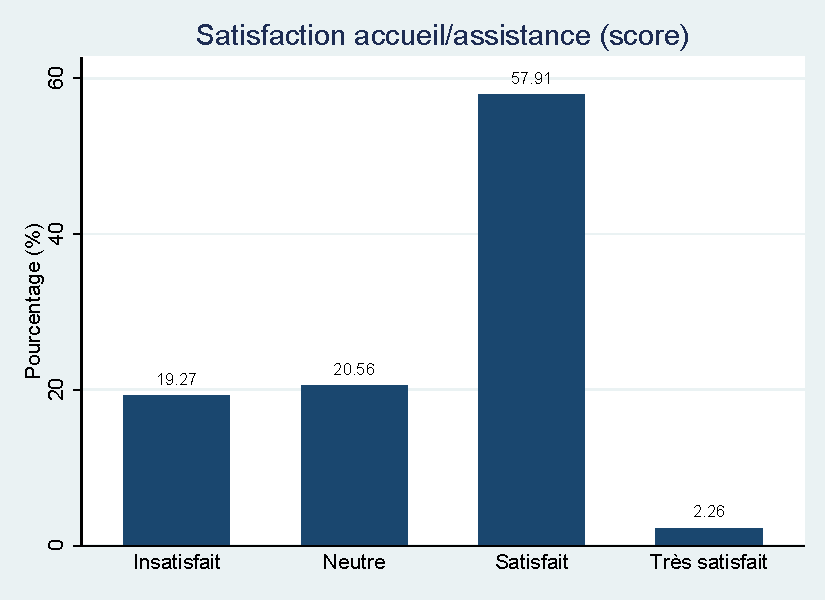
\includegraphics[width=0.6\textwidth]{../output/figures/Question_2/bar_adm_s_acceuil.pdf}
			\caption{Satisfaction par rapport à l'accueil et l'assistance}
			\label{fig:bar_acceui}
		\end{figure}
		L’analyse de la satisfaction des étudiants vis-à-vis des services d’accueil et d’assistance montre qu’une majorité relative des enquêtés se déclare satisfaite (57,91\%). Par ailleurs, 20,56\% des étudiants adoptent une position neutre, tandis que 19,27\% expriment une insatisfaction. La proportion d’étudiants très satisfaits demeure marginale, représentant seulement 2,26 \% des répondants.
		
		
		\subsubsection{Analyse des affirmations sp\'ecifiques}
		\begin{figure}[H]
			\centering
			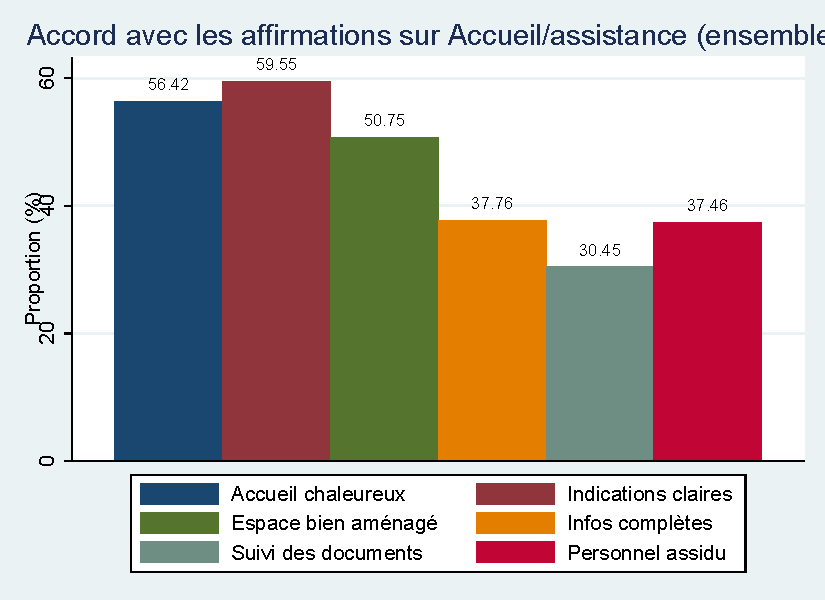
\includegraphics[width=0.6\textwidth]{../output/figures/Question_2/bar_adm_p_acceuil.pdf}
			\caption{Proportion d'accord avec les affirmations sur l'accueil et l'assistance}
			\label{fig:bar_acceui}
		\end{figure}
		\vspace{-6pt}
		Ce graphique en barres présente les proportions d’accord des étudiants avec diverses affirmations relatives à l’accueil et l’assistance. Les “Indications claires” enregistrent le taux d’accord le plus élevé avec 59,55\%. L’« Accueil chaleureux » obtient 56,42\% d’accord. L’« Espace bien aménagé » représente 50,75\% d’accord. Les « Infos complètes » constituent 37,76\% d’accord. Le « Personnel assidu » enregistre 37,46\% d’accord. Le « Suivi des documents » obtient le taux le plus faible avec 30,45\% d’accord.
		
		\subsection{Niveau global de satisfaction par rapport au processus d'inscriptions et de réinscriptions}
		
		
		\begin{figure}[H]
			\centering
			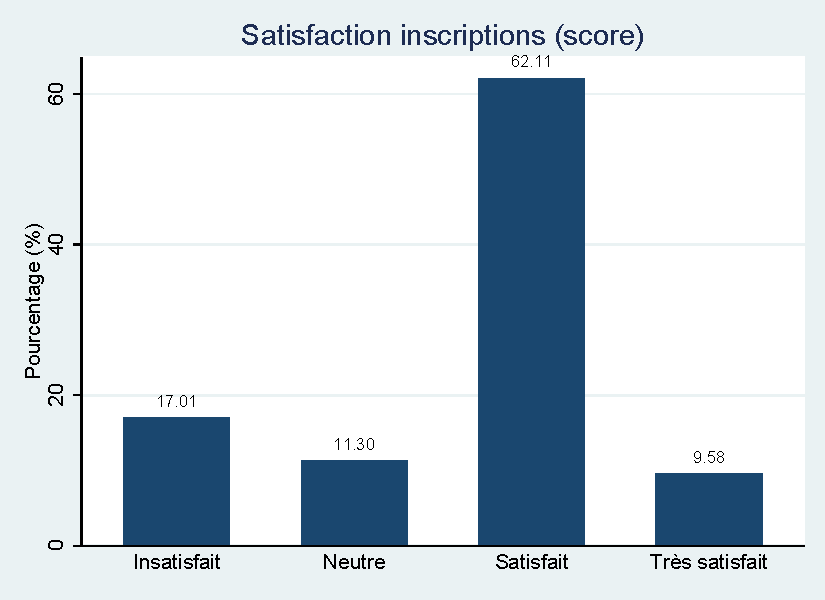
\includegraphics[width=0.6\textwidth]{../output/figures/Question_2/bar_adm_s_inscription.pdf}
			\caption{Satisfaction par rapport au processus d'inscriptions et de réinscriptions}
			\label{fig:bar_inscription}
		\end{figure}
		Les résultats indiquent que les services d’inscription constituent le domaine présentant le niveau de satisfaction le plus élevé. En effet, environ 62,11\% des étudiants déclarent en être satisfaits. À l’inverse, 17,01 \% manifestent une insatisfaction, tandis que 11,30\% se situent dans une position neutre. Par ailleurs, 9,58 \% des étudiants se déclarent très satisfaits.
		
		
		\subsubsection{Analyse des affirmations sp\'ecifiques}
		\begin{figure}[H]
			\centering
			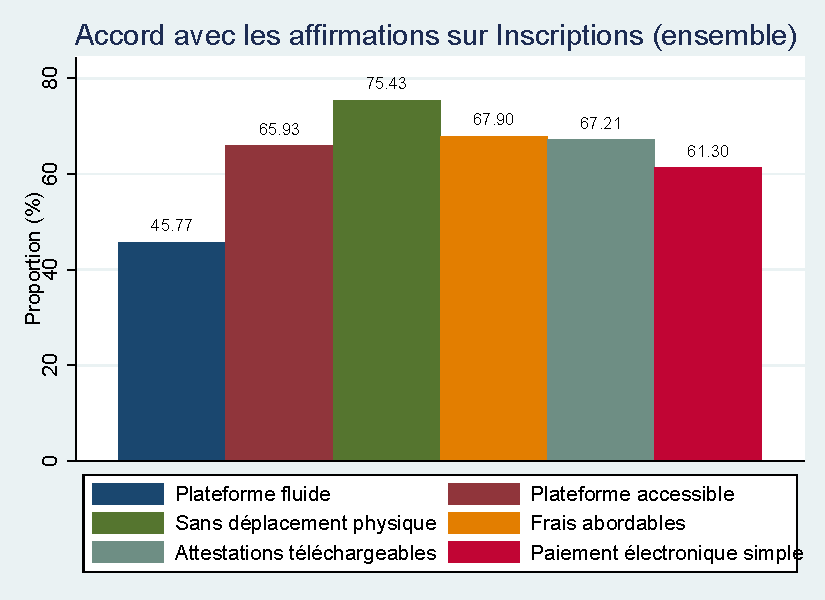
\includegraphics[width=0.6\textwidth]{../output/figures/Question_2/bar_adm_p_inscription.pdf}
			\caption{Proportion d'accord avec les affirmations par rapport au processus d'inscription}
			\label{fig:bar_inscrip}
		\end{figure}
		\vspace{-6pt}
		
		Ce graphique en barres illustre les proportions d’accord des étudiants avec diverses affirmations relatives aux inscriptions. Les “Attestations téléchargeables” enregistrent le taux d’accord le plus élevé avec 75,43\%. Les “Frais abordables” obtiennent 67,9\% d’accord. Le “Sans déplacement physique” représente 67,21\% d’accord. La “Plateforme accessible” constitue 65,93\% d’accord. Le “Paiement électronique simple” enregistre 61,3\% d’accord. La “Plateforme fluide” obtient le taux le plus faible avec 45,77\% d’accord.
		
		
		\subsection{Niveau global de satisfaction par rapport au délai de délivrance des documents au sein de l'administration}
		
		\begin{figure}[H]
			\centering
			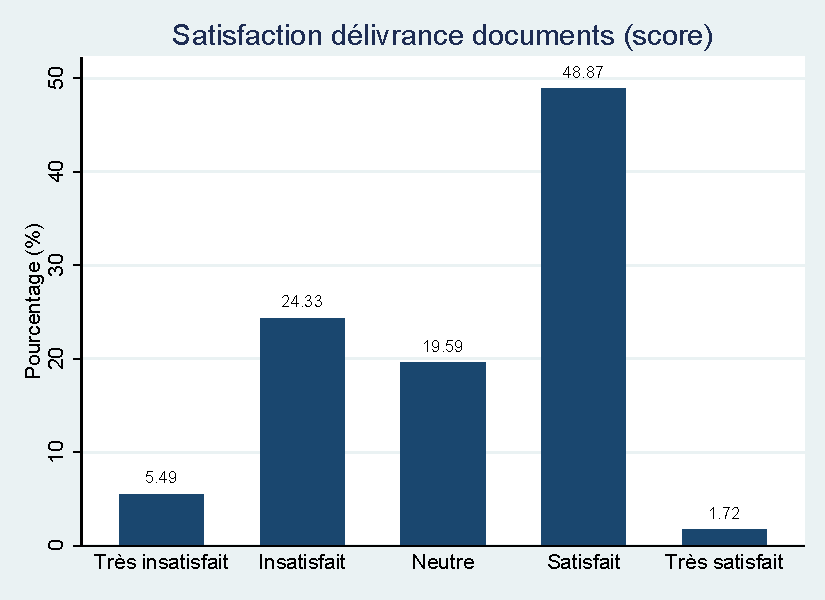
\includegraphics[width=0.6\textwidth]{../output/figures/Question_2/bar_adm_s_documents.pdf}
			\caption{Satisfaction par rapport délai de délivrance des documents au sein de l'administration}
			\label{fig:bar_acceui}
		\end{figure}
		Concernant la délivrance des documents administratifs, près de la moitié des étudiants (48,87\%) se disent satisfaits du service. Toutefois, une part non négligeable exprime des réserves : 24,33\% des étudiants se déclarent insatisfaits et 19,59 \% adoptent une position neutre. En outre, 5,49\% se disent très insatisfaits, tandis que seulement 1,72\% se déclarent très satisfaits.
		
		\subsubsection{Analyse des affirmations sp\'ecifiques}
		\begin{figure}[H]
			\centering
			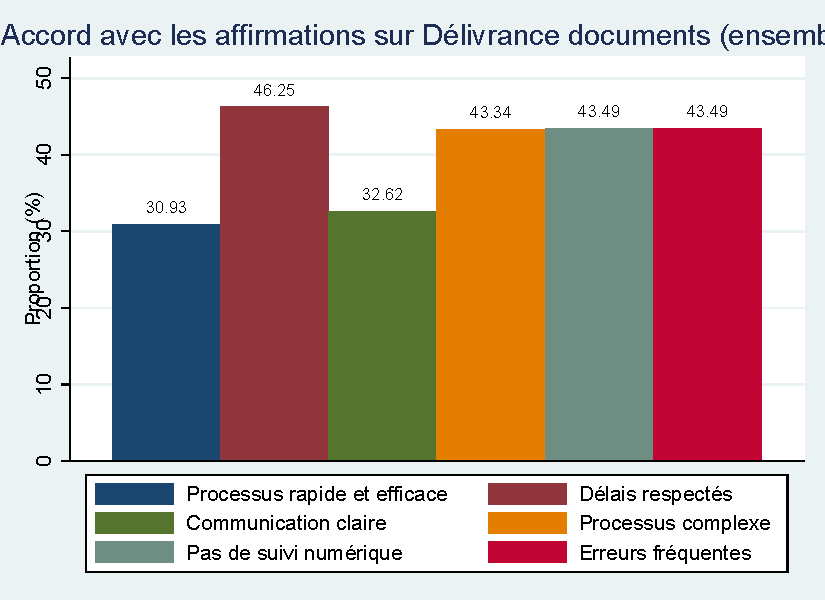
\includegraphics[width=0.6\textwidth]{../output/figures/Question_2/bar_adm_p_documents.pdf}
			\caption{Proportion d'accord avec les affirmations par rapport au délai de délivrance des documents au sein de l'administration}
			\label{fig:bar_doc}
		\end{figure}
		\vspace{-6pt}
		
		À la lecture du graphique ci-dessus, qui présente les proportions d’accord des étudiants avec diverses affirmations relatives à la délivrance de documents, on observe que les “Délais respectés” enregistrent le taux d’accord le plus élevé avec 46,25\%. Les “Erreurs fréquentes”, le “Pas de suivi numérique” et le “Processus complexe” obtiennent des taux d’accord similaires, respectivement 43,49\%, 43,49\% et 43,34\%. La “Communication claire” représente 32,62\% d’accord. Le “Processus rapide et efficace” enregistre le taux le plus faible avec 30,93\% d’accord.
		
		\subsection{Niveau global de satisfaction par rapport à la communication et l'accessibilité des informations}
		
		
		\begin{figure}[H]
			\centering
			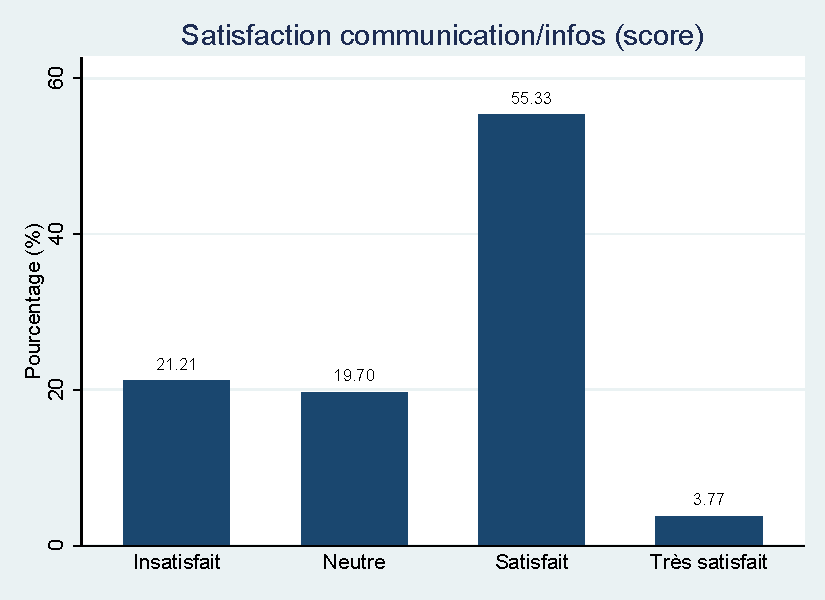
\includegraphics[width=0.6\textwidth]{../output/figures/Question_2/bar_adm_s_informations.pdf}
			\caption{Satisfaction par rapport à la communication et l'accessibilité des informations}
			\label{fig:bar_info}
		\end{figure}
		L’évaluation des services de communication et d’information révèle qu’une majorité des étudiants (55,33 \%) se déclare satisfaite. Par ailleurs, 19,70 \% adoptent une position neutre et 21,21 \% expriment une insatisfaction. La proportion d’étudiants très satisfaits reste relativement faible, s’établissant à 3,77 \%.
		
		
		\subsubsection{Analyse des affirmations sp\'ecifiques}
		\begin{figure}[H]
			\centering
			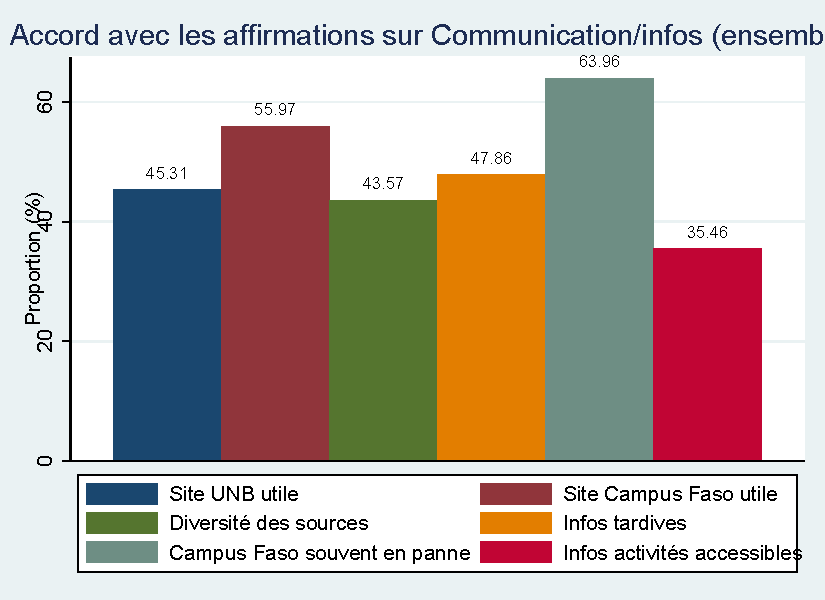
\includegraphics[width=0.6\textwidth]{../output/figures/Question_2/bar_adm_p_informations.pdf}
			\caption{Proportion d'accord avec les affirmations par rapport à la communication et l'accessibilité des informations}
			\label{fig:bar_info}
		\end{figure}
		\vspace{-6pt}
		
		Ce graphique en barres illustre les proportions d’accord des étudiants avec diverses affirmations relatives à la communication et aux informations. Le “Campus Faso souvent en panne” enregistre le taux d’accord le plus élevé avec 63,96\%. Le “Site Campus Faso utile” obtient 55,97\% d’accord. Les “Infos tardives” représentent 47,86\% d’accord. Le “Site UNB utile” constitue 45,31\% d’accord. La “Diversité des sources” enregistre 43,57\% d’accord. Les “Infos activités accessibles” obtiennent le taux le plus faible avec 35,46\% d’accord.
		
		\subsection{Niveau global de satisfaction par rapport au service sécuritaire mis à la disposition des étudiants}
		
		\begin{figure}[H]
			\centering
			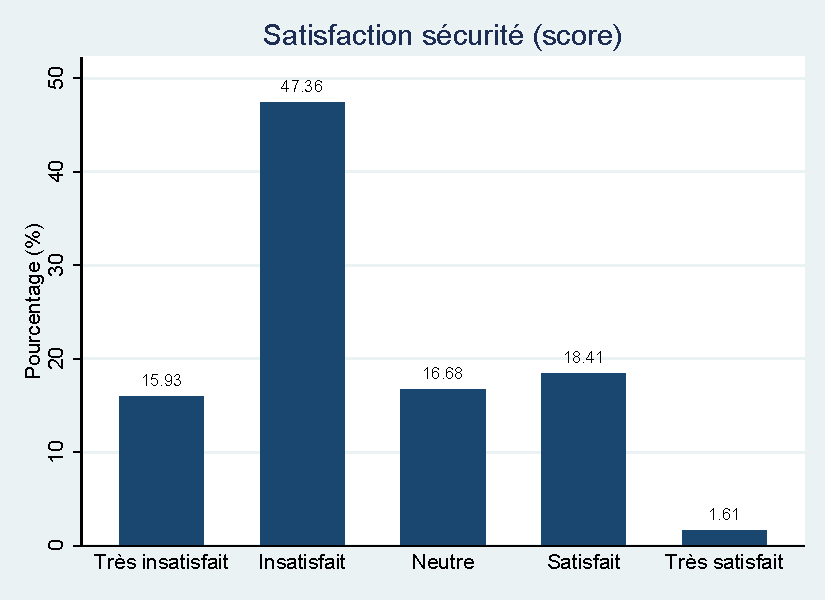
\includegraphics[width=0.6\textwidth]{../output/figures/Question_2/bar_adm_s_securite.pdf}
			\caption{Satisfaction par rapport au service sécuritaire mis à la disposition des étudiants}
			\label{fig:bar_securite}
		\end{figure}
		L’analyse de la perception de la sécurité sur le campus met en évidence une tendance majoritairement négative. En effet, 47,36\% des étudiants se déclarent insatisfaits de la situation sécuritaire, constituant la proportion la plus importante. De plus, 15,93 \% se disent très insatisfaits, tandis que 16,68 \% adoptent une position neutre. À l’inverse, seulement 18,41 \% des étudiants se déclarent satisfaits et 1,61 \% très satisfaits.
		
		
		\subsubsection{Analyse des affirmations sp\'ecifiques}
		
		\begin{figure}[H]
			\centering
			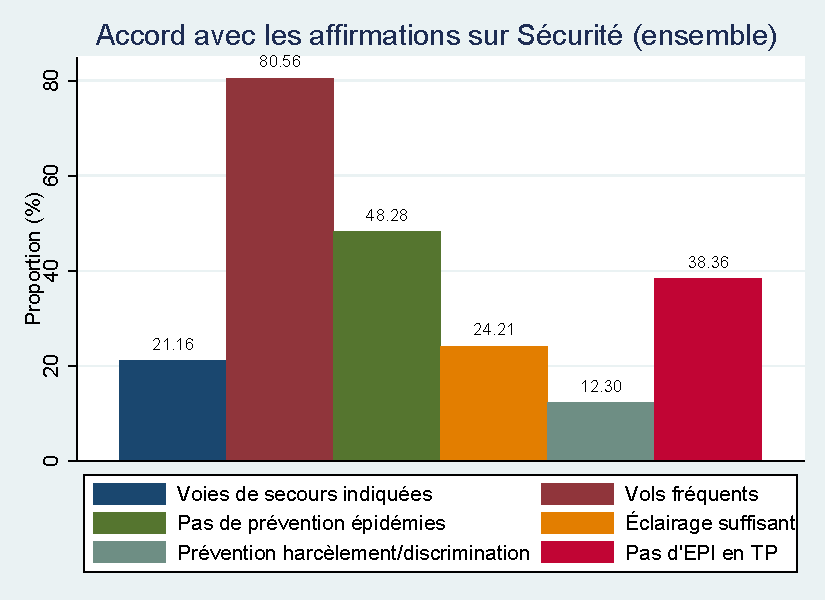
\includegraphics[width=0.6\textwidth]{../output/figures/Question_2/bar_adm_p_securite.pdf}
			\caption{Proportion d'accord avec les affirmations par rapport  au service sécuritaire mis à la disposition des étudiants}
			\label{fig:bar_securite}
		\end{figure}
		\vspace{-6pt}
		Ce graphique en barres présente les proportions d’accord des étudiants avec diverses affirmations relatives à la sécurité. Les “Vols fréquents” enregistrent le taux d’accord le plus élevé avec 80,56\%. Les “Pas de prévention épidémies” représentent 48,28\% d’accord. Les “Pas d’EPI en TP” constituent 38,36\% d’accord. Les “Éclairage suffisant” obtiennent 24,21\% d’accord. Les “Voies de secours indiquées” et “Prévention harcèlement/discrimination” enregistrent respectivement 21,16\% et 12,30\% d’accord.
		
		
		\section{SATISFACTION PAR RAPPORT AUX SERVICES
			P\'EDAGOGIQUES}
		\label{sec:satisfaction envers les services p\'edagogiques}
		
		La pertinence des fili\`eres et la qualit\'e de la formation \`a l'UNB
		jouent un r\^ole central dans la satisfaction des \'etudiants. En effet,
		lorsque les fili\`eres correspondent aux besoins du march\'e et aux
		aspirations personnelles, les \'etudiants se sentent motiv\'es et
		confiants dans leur avenir. Une p\'edagogie de qualit\'e, des enseignants
		comp\'etents et des ressources adapt\'ees renforcent l'exp\'erience
		d'apprentissage et la valeur du dipl\^ome.
		
		\subsection{Niveau global de satisfaction par rapport à la pertinence des filières}
		
		% <-- DÉCRIRE LES RÉSULTATS CHIFFRÉS AVANT DE MONTRER LA FIGURE
		
				\begin{figure}[H]
				\centering
				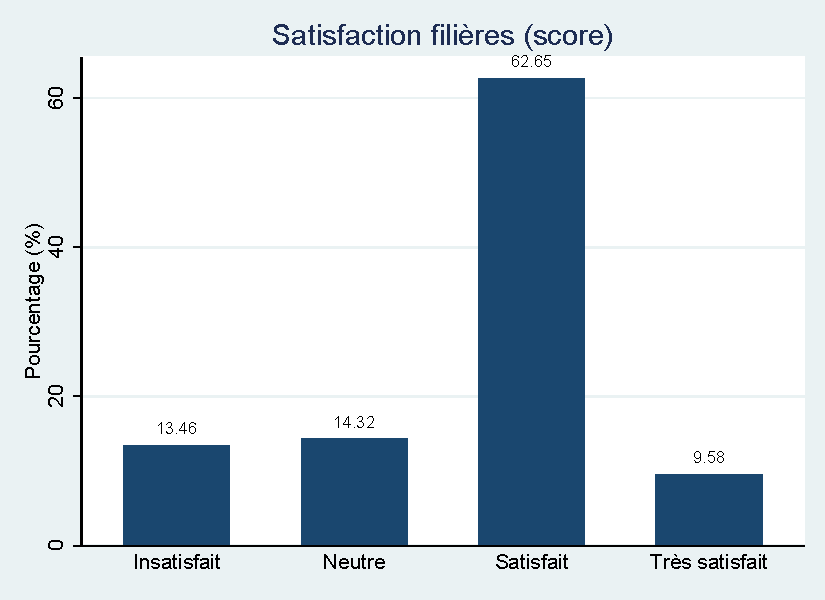
\includegraphics[width=0.6\textwidth]{../output/figures/Question_3/bar_ped_s_filieres.pdf}
				\caption{Satisfaction par rapport à la pertinence des filières proposées par l'UNB}
				\label{fig:bar_filier}
			\end{figure}
			
		% <-- INTERPRÉTER LES TABLEAUX
		L'analyse de \textbf{la figure 3.6} met en évidence que pr\`es de \textbf{6 \'etudiants sur 10} --- $62{,}65\%$ satisfaits---
		auxquels s'ajoutent $9{,}58\%$ de tr\`es satisfaits 
		appr\'ecient la pertinence des fili\`eres propos\'ees par l'UNB.
		C'est un r\'esultat encourageant, mais il masque une r\'ealit\'e
		plus nuanc\'ee~: $13{,}46\%$ des r\'epondants se d\'eclarent
		insatisfaits, et $14{,}32\%$ ne se prononcent pas clairement.
		En tout, \textbf{pr\`es de 3 \'etudiants sur 10} restent en dehors
		de la satisfaction .
		
			\begin{boiteAlerte}[Signal d'alerte]
			La pertinence des fili\`eres est le service p\'edagogique le
		mieux not\'e de l'enqu\^ete, avec un taux de satisfaction
		cumul\'e de $72{,}23\%$. En clair~: environ \textbf{7 \'etudiants
		sur 10} se disent satisfaits de l'offre de formation de l'UNB.
		\end{boiteAlerte}
		
		\subsubsection{Analyse des affirmations sp\'ecifiques}
		
		Afin d'identifier plus pr\'ecis\'ement les points forts et les points
		faibles de la pertinence des filières , les \'etudiants ont \'et\'e invit\'es \`a se prononcer sur six affirmations sp\'ecifiques. Les r\'esultats sont pr\'esent\'es dans la figure suivante.
		
		\begin{figure}[H]
			\centering
			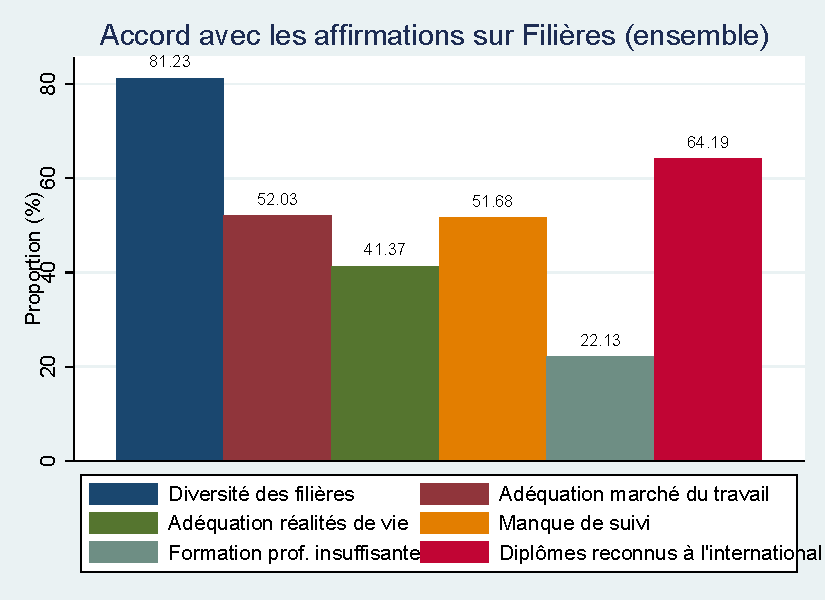
\includegraphics[width=0.6\textwidth]{../output/figures/Question_3/bar_ped_p_filieres.pdf}
			\caption{Proportion d'accord avec les affirmations sur la pertinence des filières}
			\label{fig:bar_acceuil}
		\end{figure}
		\vspace{-6pt}
		Deux points ressortent nettement de la visualisation de la figure \textbf{la figure 3.12}. D'abord, la \textbf{diversit\'e des fili\`eres}~: $81{,}23\%$ des \'etudiants la reconnaissent, un chiffre qui t\'emoigne d'une
		offre de formation r\'eelle. La \textbf{reconnaissance
		internationale des dipl\^omes} convainc \'egalement
		$64{,}19\%$ d'entre eux.

		Mais les choses se compliquent d\`es qu'on touche \`a la
		pratique. L'\textbf{ad\'equation au march\'e du travail}
		et le \textbf{suivi p\'edagogique} partagent l'opinion
		quasiment en deux ($52{,}03\%$ et $51{,}68\%$ de oui) --- ce
		qui signifie qu'un \'etudiant sur deux ne se retrouve pas
		dans ces aspects. Seuls $41{,}37\%$ estiment que les
		fili\`eres collent aux r\'ealit\'es du quotidien. Et le
		chiffre le plus parlant~: \textbf{environ $22{,}13\%$} jugent
		la formation professionnelle insuffisante. Cinq
		\'etudiants sur six ne le pensent pas.

		
		%=============================================================
		\subsection{Niveau global de satisfaction par rapport \`a la
			qualit\'e de la formation}
		%=============================================================
		\begin{figure}[H]
			\centering
			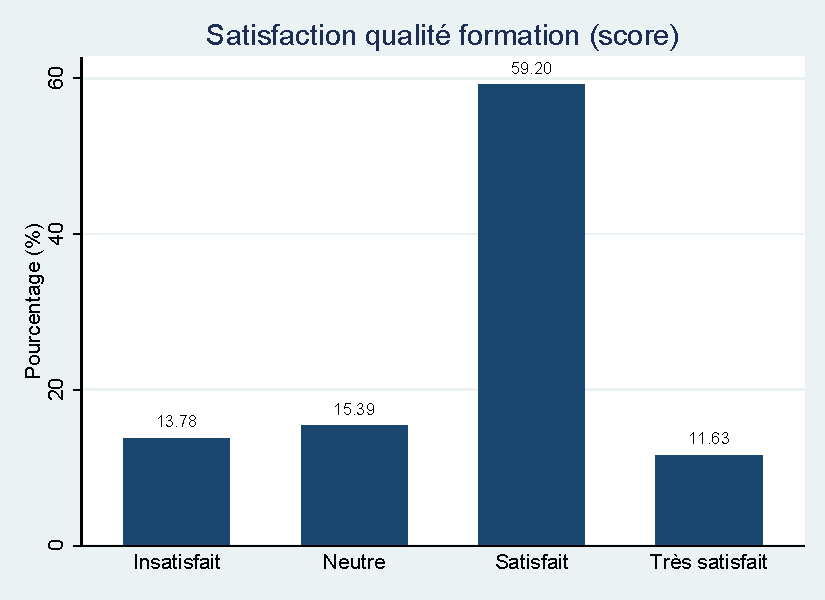
\includegraphics[width=0.6\textwidth]{../output/figures/Question_3/bar_ped_s_formation.pdf}
			\caption{Satisfaction par rapport \`a
				la qualit\'e de la formation}
			\label{fig:bar_acceuil}
		\end{figure}
		
		$59{,}2\%$ des \'etudiants se disent satisfaits de la
		qualit\'e de la formation, et $11{,}63\%$ poussent jusqu'\`a
		\textbf{tr\`es satisfaits}. C'est une majorit\'e, et elle
		compte. Mais moins d'\textbf{un \'etudiant sur trois}
		($29{,}2\%$ cumul\'es) exprime une insatisfaction ou
		s'abstient de trancher.
		
		\subsubsection{Analyse des affirmations sp\'ecifiques}
		
		Les \'etudiants se sont prononc\'es sur six affirmations
		sp\'ecifiques relatives \`a la qualit\'e de la formation.
		
		\begin{figure}[H]
			\centering
			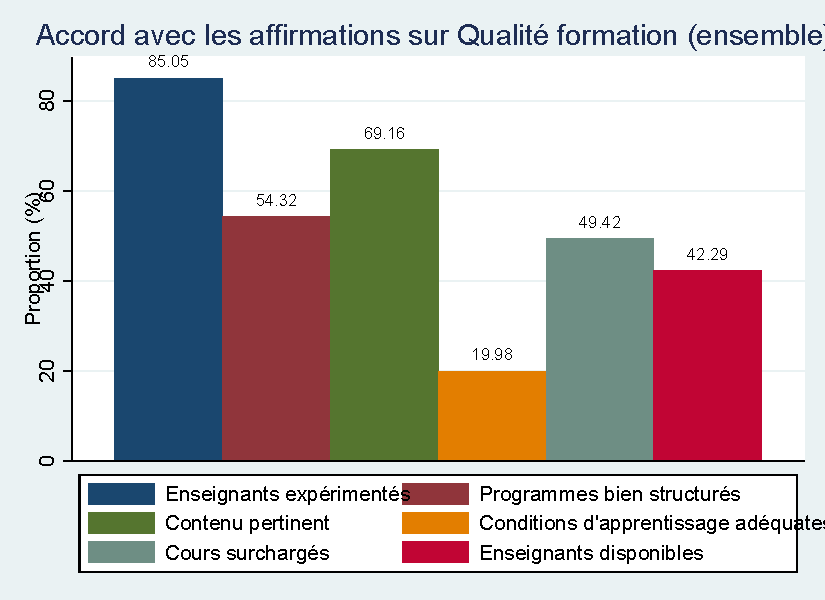
\includegraphics[width=0.6\textwidth]{../output/figures/Question_3/bar_ped_p_formation.pdf}
			\caption{Proportion d'accord avec les affirmations sur la qualit\'e
				de la formation}
			\label{fig:bar_acceuil}
		\end{figure}
		\vspace{-6pt}
		L'aspect qui fait le plus l'unanimit\'e, c'est
		\textbf{l'exp\'erience des enseignants}~: $85{,}05\%$ des
		\'etudiants leur font confiance sur ce point. Le
		\textbf{contenu pertinent des cours} et la \textbf{structuration
		des programmes} suivent avec $69{,}16\%$ et $54{,}32\%$
		de satisfaits.

		C'est au-del\`a que les choses se d\'egradent.
		\textbf{La surcharge des cours} est signal\'ee
		par pr\`es d'un \'etudiant sur deux ($49{,}4\%$).
		\textbf{L'acc\`es aux enseignants} ne satisfait
		que $42{,}3\%$ des r\'epondants. Le chiffre le
		plus inqui\'etant reste celui-ci~: \textbf{seulement
		un \'etudiant sur cinq} juge les conditions
		d'apprentissage sont vraiment ad\'equates.
		
		
		
		%=============================================================
		\subsection{Niveau global de satisfaction par rapport au service
			de gestion des stages}
		%=============================================================
		
		\begin{figure}[H]
			\centering
			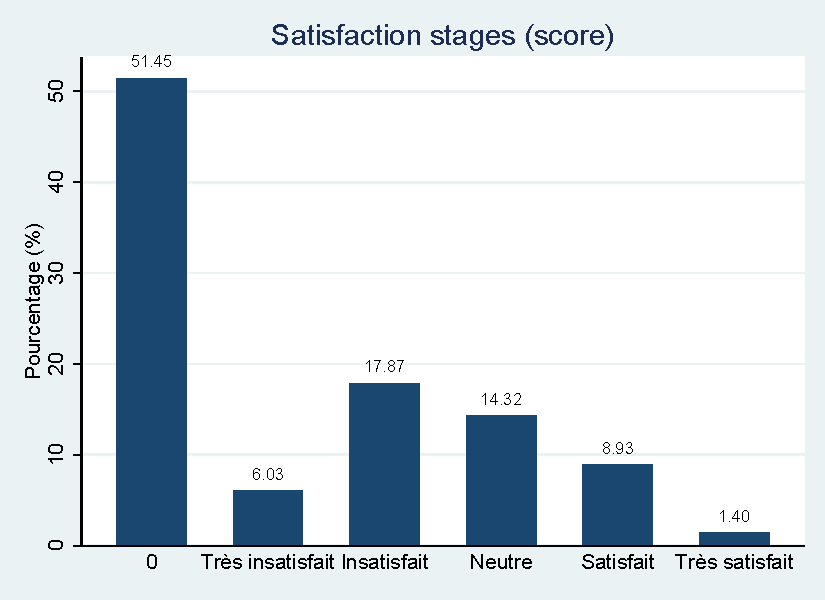
\includegraphics[width=0.6\textwidth]{../output/figures/Question_3/bar_ped_s_stages.pdf}
			\caption{Satisfaction par rapport au service de gestion des
				stages \`a l'UNB}
			\label{fig:bar_acceuil}
		
		\end{figure}
		\vspace{-6pt}
		
		Avant m\^eme d'interpr\'eter les chiffres de satisfaction, un
		fait s'impose~: \textbf{plus d'un \'etudiant sur deux}
		($51{,}45\%$) d\'eclare que ce service n'est tout simplement
		pas disponible dans son \'etablissement. Parmi ceux qui y
		ont acc\`es, $23{,}9\%$ se disent insatisfaits ou tr\`es
		insatisfaits. Seuls \textbf{$10{,}3\%$} --- moins d'un
		sur dix --- expriment une satisfaction.
		
		\begin{boiteAlerte}[Signal d'alerte]
			Le service des stages enregistre le taux de satisfaction
		le plus bas de toute la section p\'edagogique~: \textbf{un
		seul \'etudiant sur dix} s'en d\'eclare satisfait.
		Un bilan qui devrait, \`a lui seul, d\'eclencher
		une r\'eflexion urgente sur l'encadrement des
		stages \`a l'UNB.
		\end{boiteAlerte}
		
		\subsubsection{Analyse des affirmations sp\'ecifiques}
	
		\begin{figure}[H]
			\centering
			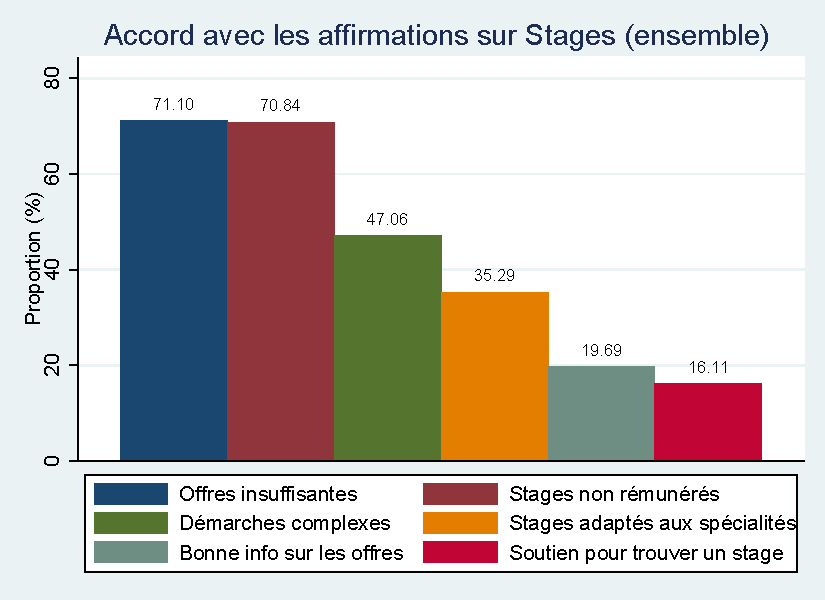
\includegraphics[width=0.6\textwidth]{../output/figures/Question_3/bar_ped_p_stages.pdf}
			\caption{Proportion d'accord avec les affirmations sur le service
				de gestion des stages}
			\label{fig:bar_acceuil}
		\end{figure}
		\vspace{-6pt}
		\textbf{La figure 3.16} présente un service au bord de l'implosion.
		\textbf{7 \'etudiants sur 10} d\'enoncent l'insuffisance
		des offres de stages par l'UNB ($71{,}1\%$) et l'absence de r\'emun\'eration d\'enonc\'ee par ($70{,}84\%$) des \'etudiants. Pr\`es
		d'un sur deux ($47{,}06\%$) juge les d\'emarches
		administratives  pour accéder aux stages trop lourdes. Seul un tiers pense
		que le stages propos\'es correspondent vraiment \`a
		sa sp\'ecialit\'e. Moins d'une personne sur cinq
		d\'eclare \^etre inform\'ee des offres disponibles,
		et seulement $16{,}11\%$ se sentent accompagn\'es
		dans leur recherche de stage.
		
		
		%=============================================================
		\subsection{Niveau global de satisfaction par rapport au
			traitement des r\'eclamations}
		%=============================================================
		
		\begin{figure}[H]
			\centering
			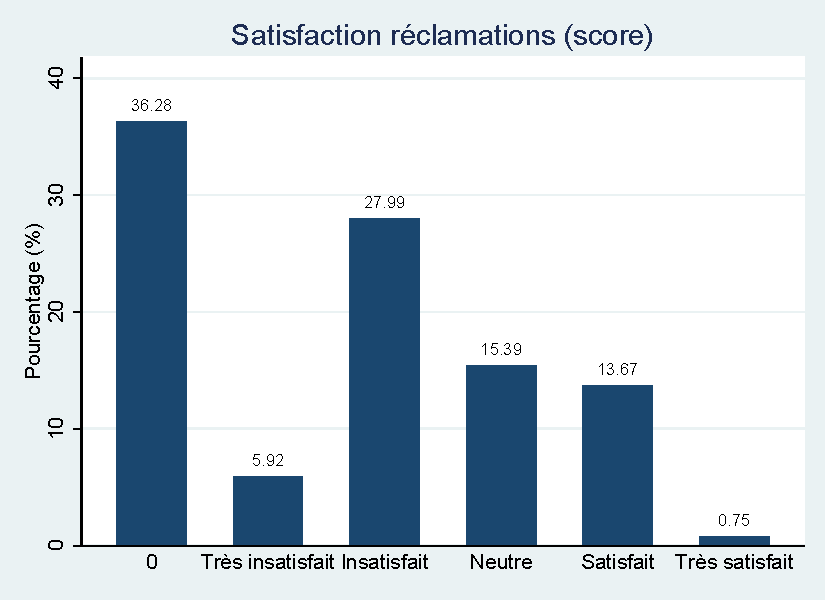
\includegraphics[width=0.6\textwidth]{../output/figures/Question_3/bar_ped_s_reclamations.pdf}
			\caption{Satisfaction par rapport au traitement des
				r\'eclamations \`a l'UNB}
			\label{fig:bar_acceuil}
	
		\end{figure}
		
		
		$36{,}28\%$ des \'etudiants d\'eclarent que ce service
		n'existe pas dans leur \'etablissement. Pour ceux
		qui y ont eu recours, le bilan est d\'ecevant~:
		pr\`es d'\textbf{un \'etudiant sur trois} se dit
		insatisfait ou très insatisfaits, et seuls $14{,}4\%$ (cumuls) en sont satisfaits.
	
		\subsubsection{Analyse des affirmations sp\'ecifiques}
		
		\begin{figure}[H]
			\centering
			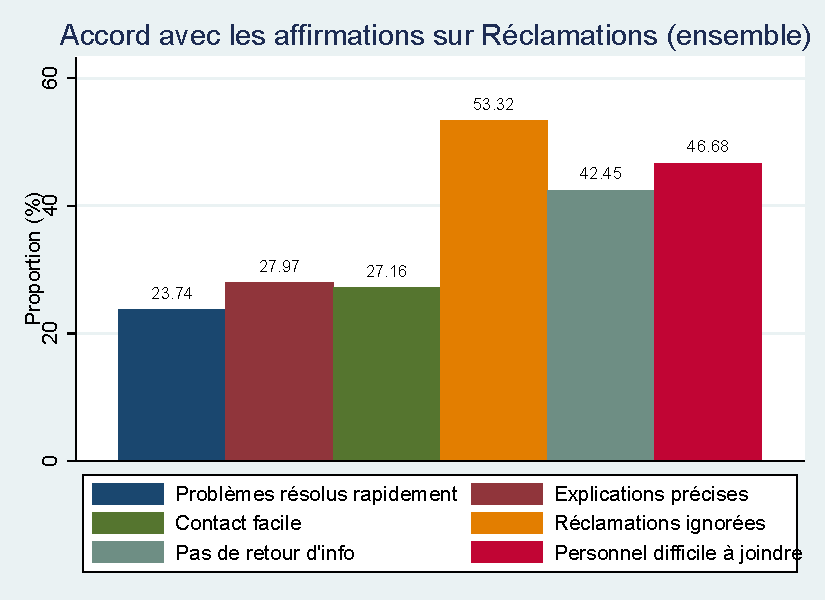
\includegraphics[width=0.6\textwidth]{../output/figures/Question_3/bar_ped_p_reclamations.pdf}
			\caption{Proportion d'accord avec les affirmations sur le
				traitement des r\'eclamations }
			\label{fig:bar_acceuil}
		\end{figure}
		\vspace{-6pt}
		Le constat est brutal~: \textbf{plus d'un \'etudiant sur
		deux} ($53{,}3\%$) a le sentiment que ses r\'eclamations
		sont tout simplement ignor\'ees. Joindre le personnel
		rel\`eve du parcours du combattant pour $46{,}68\%$
		d'entre eux, et $42{,}45\%$ ne re\c{c}oivent aucun
		retour sur leur dossier. Du c\^ot\'e positif, les
		chiffres sont maigres~: moins d'un \'etudiant sur
		dix seulement d\'eclare recevoir des explications
		claires ($27{,}97\%$), contacter facilement les enseignants ou le personnel administratif est une autre lutte pour $27{,}16\%$ des étudiants.Seulement $23{,}74\%$ sont satisfaits de la rapidité à laquelle leurs problèmes sont résolus au sein de l'UNB.  
		
		
		
		%=============================================================
		\subsection{Niveau global de satisfaction par rapport au
			service de la biblioth\`eque}
		%=============================================================
		
		
	
		\begin{figure}[H]
			\centering
			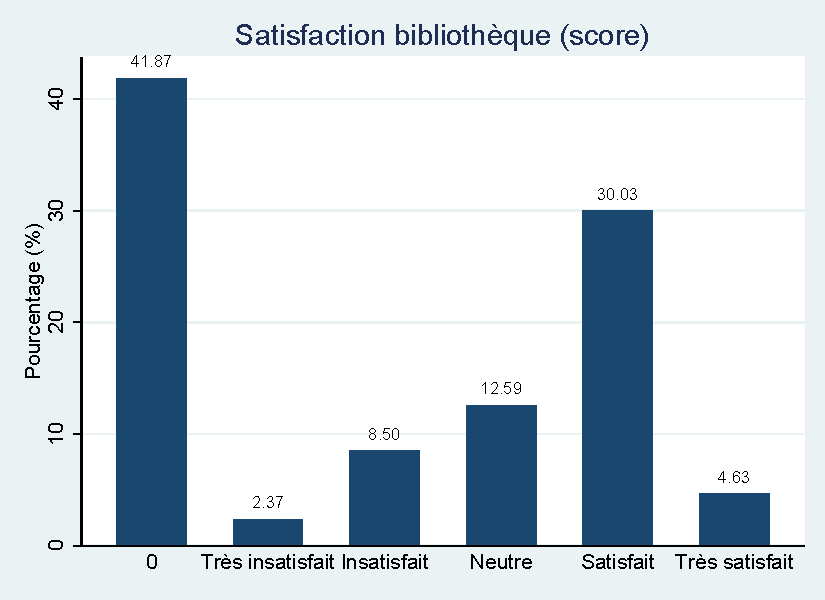
\includegraphics[width=0.6\textwidth]{../output/figures/Question_3/bar_ped_s_bibliotheque.pdf}
			\caption{Satisfaction par rapport au service de la biblioth\`eque
				\`a l'UNB}
			\label{fig:bar_acceuil}
		\end{figure}
		\vspace{-6pt}
		
		La r\'epartition des r\'eponses montre que
		$34{,}66\%$ des \'etudiants se d\'eclarent
		\textbf{satisfaits ou tr\`es satisfaits} du service
		de la biblioth\`eque. \`A l'oppos\'e, $10{,}87\%$
		expriment une insatisfaction et $12{,}59\%$ restent
		neutres. Il est \`a noter que pr\`es de
		\textbf{4 \'etudiants sur 10} ($41{,}87\%$) ont
		indiqu\'e que ce service ne leur est pas applicable
	
		
		\subsubsection{Analyse des affirmations sp\'ecifiques}
		
		\begin{figure}[H]
			\centering
			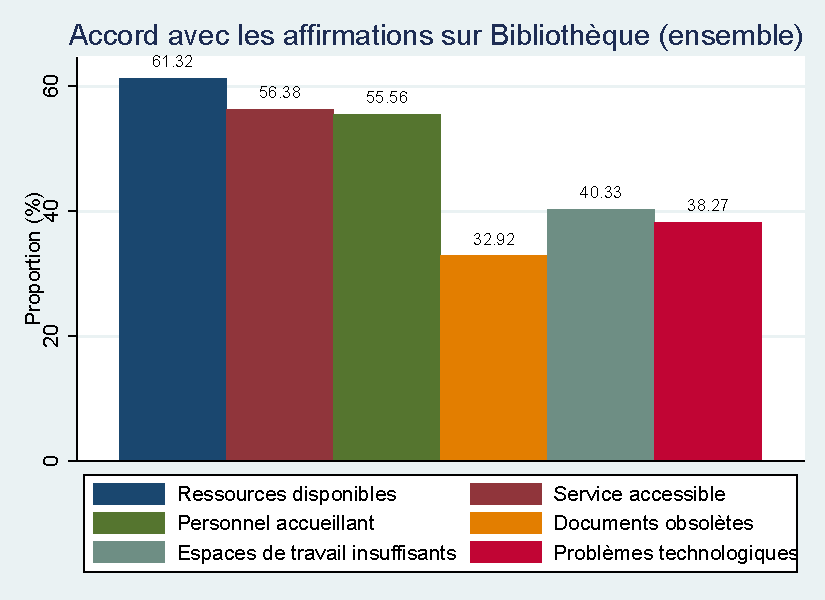
\includegraphics[width=0.6\textwidth]{../output/figures/Question_3/bar_ped_p_bibliotheque.pdf}
			\caption{Proportion d'accord avec les affirmations sur le service
				de la biblioth\`eque}
			\label{fig:bar_acceuil}
		\end{figure}
		\vspace{-6pt}
		La biblioth\`eque a ses atouts, et ils sont r\'eels. Les
		\textbf{ressources sont jug\'ees disponibles} par $61{,}32\%$
		des \'etudiants, \textbf{le service accessible} par $56{,}38\%$,
		et \textbf{l'accueil du personnel} appr\'eci\'e par $55{,}56\%$.

		Mais le revers est tout aussi net. Pr\`es de
		\textbf{4 \'etudiants sur 10} signalent des insuffisances
		technologiques ($38{,}27\%$) et des espaces de travail
		trop \'etroits ($40{,}33\%$). Ce qui retient le plus
		l'attention, c'est le chiffre sur l'actualit\'e des
		fonds documentaires~: \textbf{un \'etudiant sur trois}
		($32{,}9\%$) estime que les documents sont p\'erim\'es.
	
		\begin{boiteResultat}[Bilan du service p\'edagogique]
			\begin{itemize}[itemsep=3pt]
				\item \textbf{Meilleur service}~: La diversité des filières proposées par l'UNB avec une satisfaction d'environ
				$72{,}2\%$.
				\item \textbf{Service le plus critiqu\'e}~: Le service par rapport à la gestion des stages avec une satisfaction d'environ ($10{,}33\%$). 
				\item \textbf{Probl\`eme transversal}~: Contrairement à la satisfaction de la qualité des formation et par rapport au service de la bibliothèque, le service par rapport au traitement des réclamations présente une satisfaction faible. En effet environ une seule personne sur sept présente une satisfaction par rapport à ce service.  
			\end{itemize}
		\end{boiteResultat}
		
		\subsection{Satisfaction des services p\'edagogiques par rapport aux \'etabissements}
		
		Afin de v\'erifier si la satisfaction p\'edagogique varie d'un
		\'etablissement \`a l'autre, des boites à moustache ont \'et\'e construits
		\`a partir des cinq sections p\'edagogiques \'evalu\'ees.
		Les r\'esultats sont pr\'esent\'es ci-dessous:
		
		\begin{figure}[H]
			\centering
			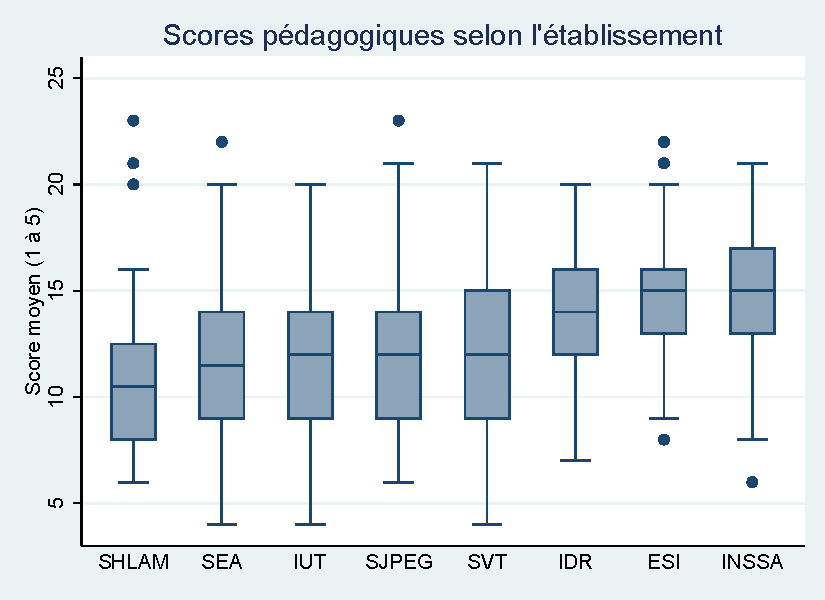
\includegraphics[width=0.6\textwidth]{../output/figures/Question_3/box_score_ped_etb.pdf}
			\caption{Satisfaction des services p\'edagogiques par rapport aux \'etabissements}
			\label{fig:bar_acceuil}
		\end{figure}
				\vspace{-6pt}
				La figure r\'ev\`ele d'embl\'ee des niveaux de satisfaction
		in\'egaux selon les \'etablissements. L'\textbf{INSSA} et
		l'\textbf{ESI} se d\'etachent avec les m\'edianes les plus
		\'elev\'ees, t\'emoignant d'une satisfaction p\'edagogique
		g\'en\'eralement plus marqu\'ee dans ces structures.
		\`A l'oppos\'e, \textbf{SHLAM} et \textbf{SEA} affichent
		les m\'edianes les plus basses --- leurs \'etudiants sont,
		en majorit\'e, moins satisfaits des services p\'edagogiques.
		La taille des bo\'ites est g\'en\'eralement contenue, ce
		qui traduit une relative homog\'en\'eit\'e des avis au sein
		de chaque \'etablissement. Seul \textbf{SVT} fait exception~:
		sa bo\'ite plus large indique que les \'etudiants y ont des
		avis beaucoup plus partag\'es sur la qualit\'e du service.

		Ces diff\'erences visuelles sont-elles r\'eellement
		significatives~? Un \textbf{test de Kruskal-Wallis} r\'epond
		par l'affirmative ($p < 0{,}001$)~: l'\'etablissement
		d'appartenance influence bel et bien la satisfaction
		p\'edagogique. Des tests post-hoc de Mann-Whitney ont
		ensuite permis de localiser les \'ecarts. Sur les
		\textbf{28 paires} possibles, \textbf{10 sont significatives}
		au seuil de $5\%$, toutes impliquant soit
		l'\textbf{INSSA} (le plus satisfait) soit
		\textbf{SHLAM} (le moins satisfait).
		
		L'ensemble de ces r\'esultats d\'esigne \textbf{SHLAM}
		comme l'\'etablissement dont les \'etudiants sont les
		moins satisfaits des services p\'edagogiques~: cinq
		comparaisons sur dix l'impliquent comme le groupe
		le moins bien not\'e. \`A l'inverse, \textbf{INSSA} se
		d\'emarque positivement dans toutes les paires o\`u
		il appara\'\i t.
		
		\subsection{Satisfaction des services p\'edagogiques selon le niveau d'\'etude}
		
		Dans cette partie, nous analyserons le niveau de satisfaction p\'edagogique selon le niveau d'\'etude. Pour cela, des boîtes à moustaches ont été construits. 
		
		\begin{figure}[H]
		\centering
		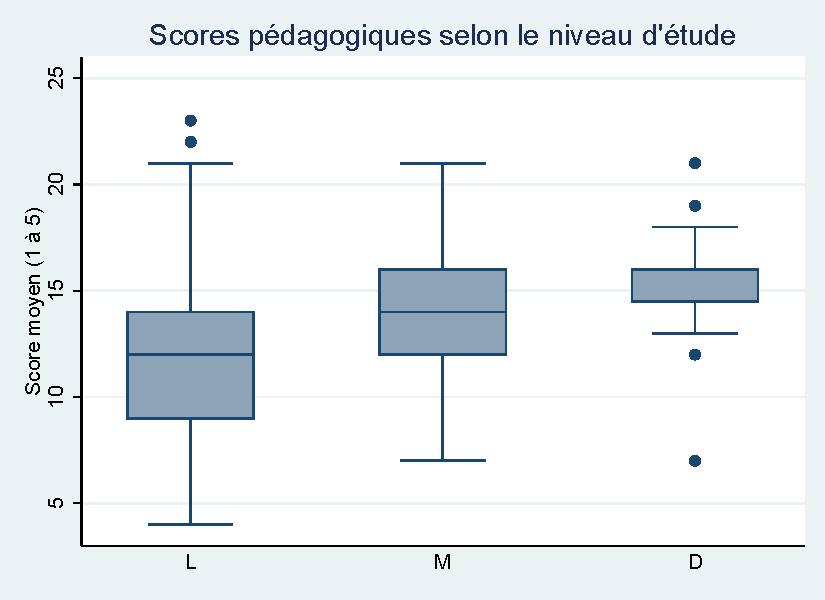
\includegraphics[width=0.6\textwidth]{../output/figures/Question_3/box_score_ped_niv_etd.pdf}
		\caption{Satisfaction des services p\'edagogiques selon le niveau d'\'etude}
		\label{fig:bar_acceuil}
	\end{figure}
		\vspace{-6pt}
		La lecture de la figure appelle plusieurs remarques.
		Les \textbf{doctorants} affichent la m\'ediane la plus
		\'elev\'ee~: ils sont globalement les plus satisfaits des
		services p\'edagogiques. Leur bo\'ite pr\'esente une
		particulier\'e~: la m\'ediane est confondue au troisi\'eme
		quartile, ce qui signifie qu'au moins \textbf{75\% d'entre
		eux n'ont pas d\'epass\'e ce niveau de satisfaction}.
		La distribution est \textbf{asym\'etrique \`a gauche}~:
		les avis n\'egatifs sont dispers\'es, tandis que les
		avis positifs sont tous concentr\'es au m\^eme niveau ---
		un plafonnement net de la satisfaction.

		Les \'etudiants en \textbf{Licence} pr\'esentent la
		m\'ediane la plus faible. Leur bo\'ite est \'egalement
		plus \'etendue dans la partie inf\'erieure, refl\'etant
		une plus grande diversit\'e d'avis parmi ceux qui se
		disent peu satisfaits. Quelques valeurs aberrantes
		\'elev\'ees indiquent cependant qu'une minorit\'e
		d'\'etudiants en Licence exprime une satisfaction
		très positive. Les \'etudiants en \textbf{Master}
		se situent dans une position interm\'ediaire, avec
		des avis relativement homog\'enes.
		
		
		
		%=============================================================
		\section{SATISFACTION PAR RAPPORT AUX SERVICES SOCIAUX}
		%=============================================================
		
		Les services sociaux repr\'esentent le quotidien de l'\'etudiant
		hors des salles de cours~: se loger, se nourrir, se soigner,
		pratiquer une activit\'e sportive ou culturelle. Dans le contexte
		d'une universit\'e comme l'UNB, o\`u beaucoup d'\'etudiants viennent
		de l'int\'erieur du pays et vivent en cit\'e universitaire avec des
		moyens limit\'es, la qualit\'e de ces services conditionne directement
		les conditions d'\'etude et le bien-\^etre g\'en\'eral.
		
		
		%=============================================================
    	\subsection{Satisfaction par rapport aux services de logement}
		%=============================================================
		
		Le logement universitaire est souvent la premi\`ere pr\'eoccupation
		de l'\'etudiant venu de la sous région. Partager une chambre, g\'erer
		l'hygiene, assurer sa s\'ecurit\'e au quotidien --- ce sont des
		r\'ealit\'es que vivent chaque jour des centaines d'\'etudiants
		de l'UNB.
		
	\begin{figure}[H]
		\centering
			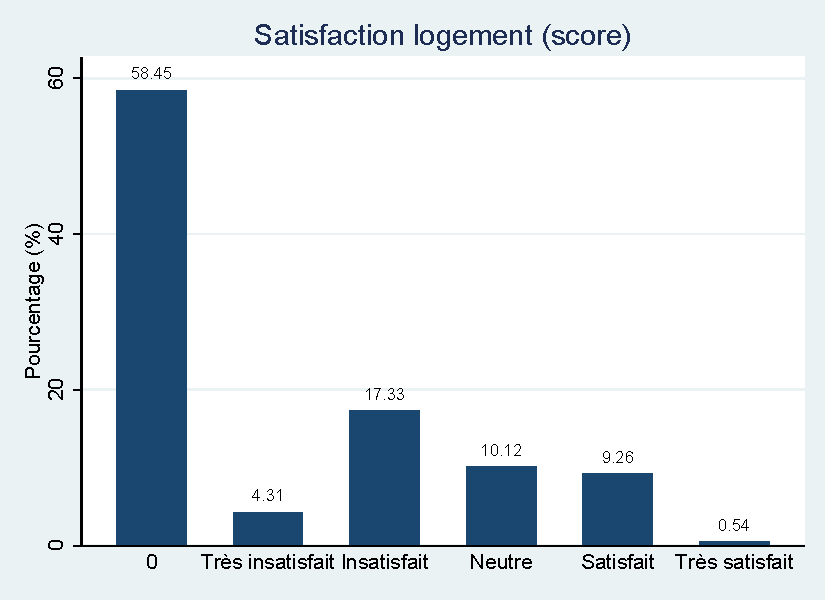
\includegraphics[width=0.6\textwidth]{../output/figures/Question_4/bar_soc_s_logement.pdf}
			\caption{Satisfaction par rapport aux services de logement}
			\label{fig:bar_logement}
	\end{figure}
	\vspace{-6pt}
	
	\textbf{Six \'etudiants sur dix} d\'eclarent que le
		logement universitaire ne les concerne pas --- ils
		ne r\'esident pas en cit\'e. Mais parmi ceux qui
		y vivent, la r\'ealit\'e est dure~: $21{,}6\%$ se
		disent insatisfaits ou tr\`es insatisfaits, et
		\textbf{seulement $9{,}8\%$} expriment une satisfaction.
		C'est le score de satisfaction le plus bas de toute
		l'enqu\^ete. Quiconque a d\'ej\`a mis les pieds dans
		une cit\'e universitaire burkinab\`e comprend vite
		pourquoi.
		
		\begin{boiteAlerte}[Signal d'alerte]
			Avec un score moyen de $1{,}09/5$ et moins de $10\%$
		de satisfaits, le logement est le \textbf{service le
		plus mal not\'e de toute l'enqu\^ete}. Ce n'est pas
		un probl\`eme de perception~: c'est un probl\`eme
		structurel qui n\'ecessite des investissements
		concrets et urgents.
		\end{boiteAlerte}
		
		\subsubsection{Analyse des affirmations sp\'ecifiques}
		
		\begin{figure}[H]
			\centering
			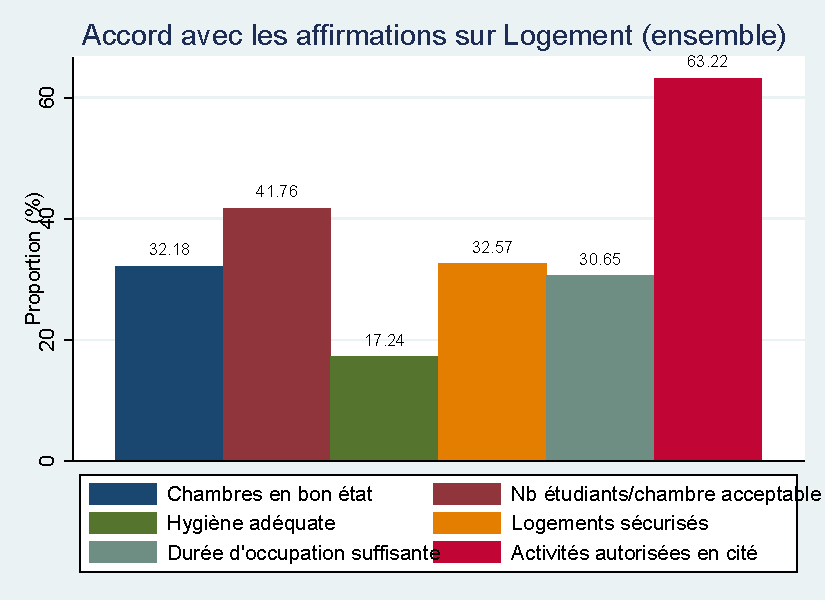
\includegraphics[width=0.6\textwidth]{../output/figures/Question_4/bar_soc_p_logement.pdf}
			\caption{Proportion d'accord avec les affirmations sur le
				logement }
			\label{fig:bar_logemen}
		\end{figure}
		\vspace{-6pt}
		
		Le seul point apprécié par la majorité est la \textbf{libert\'e
		d'exercer ses activit\'es en cit\'e}, appr\'eci\'ee par $63{,}2\%$
		des r\'esidents. En effet, seulement $\mathbf{41{,}8\%}$ jugent le \textbf{nombre d'\'etudiants par chambre acceptable} --- ce qui veut dire que la majorit\'e vit
		dans des conditions de surpopulation. Plus grave~: \textbf{moins d'un
		\'etudiant sur trois} estime que les \textbf{chambres sont en bon
		\'etat} ($32{,}2\%$), que les \textbf{logements sont s\'ecuris\'es}
		($32{,}6\%$) ou que la \textbf{dur\'ee d'occupation est suffisante}
		($30{,}7\%$).Pire, seulement $17{,}24\%$ des étudiants jugent l'hygiène dans les cités adéquate --- ce qui veut dire qu'ils vivent dans des conditions d'insalubrité. Quatre probl\`emes concrets, quotidiens, qui p\`esent lourd sur le moral et les conditions de travail des \'etudiants
		h\'eberg\'es.
		
		
		%=============================================================
		\subsection{Satisfaction par rapport aux services de sant\'e}
		%=============================================================
		
		Se soigner \`a l'universit\'e n'est pas toujours \'evident.
		Entre les consultations en dehors des heures de cours et la
		question de la disponibilit\'e du personnel m\'edical, les
		\'etudiants de l'UNB ont un avis tranch\'e sur ce sujet.
	
			\begin{figure}[H]
			\centering
				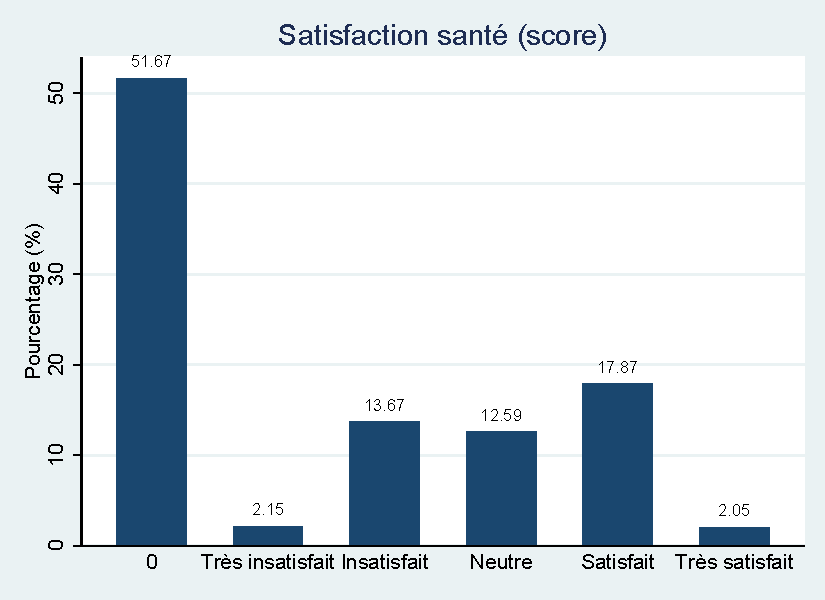
\includegraphics[width=0.6\textwidth]{../output/figures/Question_4/bar_soc_s_sante.pdf}
				\caption{Satisfaction par rapport aux services de sant\'e}
				\label{fig:bar_sante}
		
		\end{figure}
		\vspace{-6pt}
		Plus d'un \'etudiant sur deux ($51{,}7\%$) affirme
		que le service de sant\'e n'existe tout simplement
		pas dans son \'etablissement. Parmi ceux qui y ont
		acc\`es, les avis restent divis\'es~: $19{,}9\%$
		se disent satisfaits ou tr\`es satisfaits, $15{,}8\%$
		insatisfaits, et $13\%$ neutres. Une chose est claire~:
		quand on exclut les \'etudiants qui n'y ont pas acc\`es,
		le service de sant\'e de l'UNB ne convainc pas
		la majorit\'e de ses utilisateurs.
		
		\subsubsection{Analyse des affirmations sp\'ecifiques}
		
		\begin{figure}[H]
			\centering
			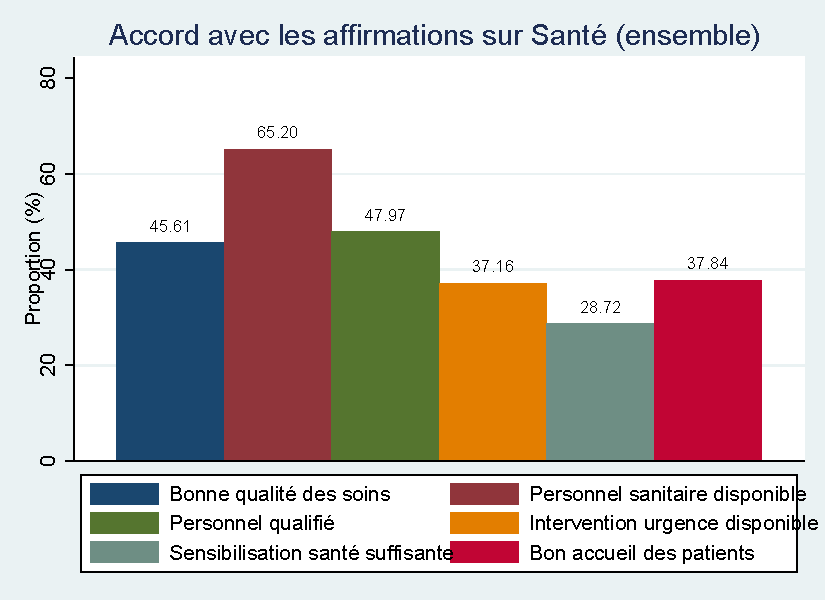
\includegraphics[width=0.6\textwidth]{../output/figures/Question_4/bar_soc_p_sante.pdf}
			\caption{Proportion d'accord avec les affirmations sur le service santé }
			\label{fig:bar_sant}
		\end{figure}
		\vspace{-6pt}
		Le point le plus solide, c'est la \textbf{pr\'esence
		du personnel}~: $65{,}2\%$ des \'etudiants confirment
		qu'il y a au moins quelqu'un \`a qui s'adresser.
		C'est un minimum, mais c'est d\'ej\`a quelque chose.

		Le probl\`eme, c'est que la pr\'esence ne suffit
		pas. La \textbf{qualification du personnel} ne
		convainc que $48\%$, et la \textbf{qualit\'e des
		soins} ne satisfait que $45{,}6\%$ --- soit moins
		d'un \'etudiant sur deux. Les lacunes les plus
		s\'erieuses se trouvent ailleurs~: les
		\textbf{interventions d'urgence} ne rassurent que
		$37{,}8\%$ des r\'epondants. La \textbf{sensibilisation
		\`a la sant\'e} est jug\'ee suffisante par \`a peine
		$28{,}7\%$ --- moins d'un \'etudiant sur trois. Dans
		un environnement expos\'e au paludisme, aux \'epid\'emies
		saisonni\`eres et au stress des examens, c'est un
		manque criant.
		
		
		%=============================================================
		\subsection{Satisfaction par rapport aux services de restauration}
		%=============================================================
		
		Le restaurant universitaire --- le \textit{RU} --- est un des
		lieux les plus fr\'equent\'es du campus. Pour beaucoup d'\'etudiants
		au budget serr\'e, c'est souvent le seul repas chaud de la journ\'ee.
		Autant dire que les attentes sont \'elev\'ees, et que la d\'eception
		peut \^etre vive.
		
			\begin{figure}[H]
			\centering
				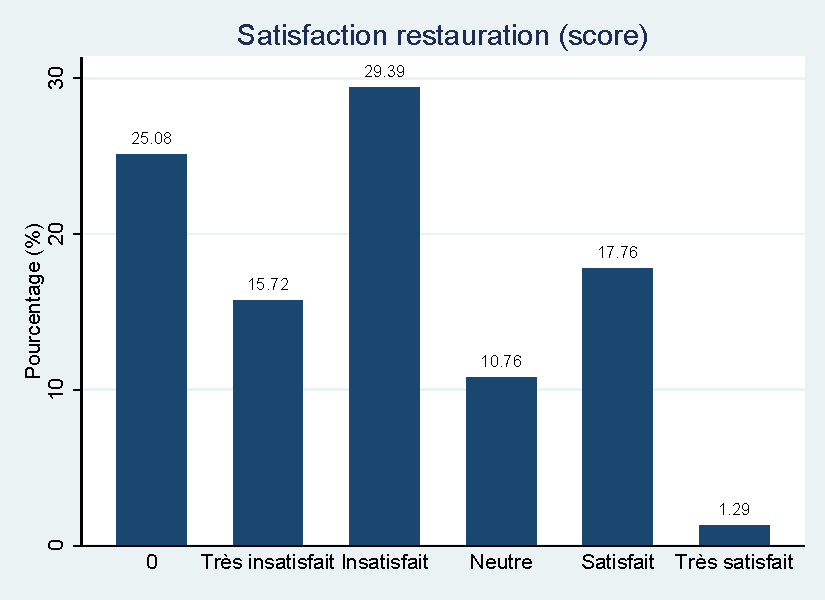
\includegraphics[width=0.6\textwidth]{../output/figures/Question_4/bar_soc_s_restau.pdf}
				\caption{Satisfaction par rapport aux services de restauration}
				\label{fig:bar_restau}
			
		\end{figure}
		\vspace{-6pt}
		
		Un quart des \'etudiants ($25{,}1\%$) d\'eclarent ne
		pas avoir acc\`es au restaurant universitaire. Parmi
		ceux qui l'utilisent, le bilan est lourd~: \textbf{pr\`es
		de la moiti\'e} ($45{,}6\%$) se disent insatisfaits ou
		tr\`es insatisfaits. Seuls $19{,}1\%$ en sont satisfaits.
		Pour un service que beaucoup d'\'etudiants fr\'equentent
		chaque jour, ces chiffres p\`esent. 
		
		\subsubsection{Analyse des affirmations sp\'ecifiques}
		
			\begin{figure}[H]
			\centering
			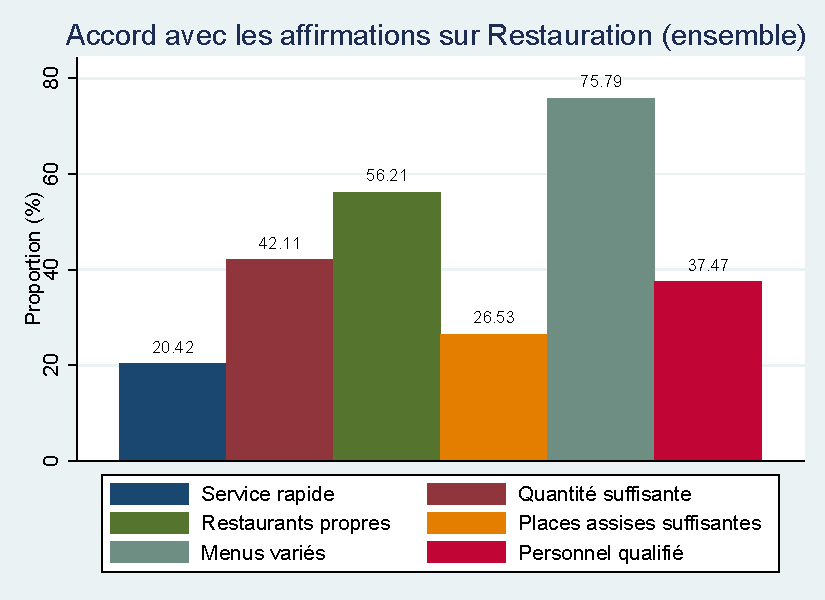
\includegraphics[width=0.6\textwidth]{../output/figures/Question_4/bar_soc_p_restau.pdf}
			\caption{Proportion d'accord avec les affirmations sur le service de la restauration }
			\label{fig:bar_resto}
		\end{figure}
		\vspace{-6pt}
		Deux points sauvent la mise. La \textbf{propret\'e}
		est jug\'ee satisfaisante par $56{,}2\%$ des \'etudiants
		--- un score correct. Et la \textbf{diversit\'e des
		menus} convainc m\^eme $75{,}8\%$ d'entre eux --- c'est
		le chiffre le plus \'elev\'e de toute la section. L'UNB
		fait donc des efforts sur ce qu'on voit.

		Le probl\`eme, c'est ce qu'on ressent en sortant.
		\textbf{La quantit\'e servie} ne satisfait que $42{,}1\%$
		des r\'epondants --- beaucoup repartent le ventre
		insuffisamment rempli. \textbf{La qualification du
		personnel} ne convainc que $37{,}5\%$. Et les deux
		points les plus critiques~: \textbf{moins d'un \'etudiant
		sur quatre} juge les places assises suffisantes ($26{,}5\%$),
		et seuls $20{,}4\%$ trouvent le service rapide.
		Attendre longtemps pour manger peu~: c'est le quotidien
		de nombreux \'etudiants au RU de l'UNB.
		
		
		%=============================================================
		\subsection{Satisfaction par rapport aux services sportifs
			et culturels}
		%=============================================================
		
		Le sport et la culture sont souvent les parents pauvres des
		universit\'es africaines, rel\'egu\'es loin derri\`ere les
		pr\'eoccupations acad\'emiques et administratives. Pourtant,
		ils jouent un r\^ole essentiel dans l'\'epanouissement personnel
		de l'\'etudiant et dans le sentiment d'appartenance \`a une
		communaut\'e universitaire.
		

		\begin{figure}[H]
		\centering
			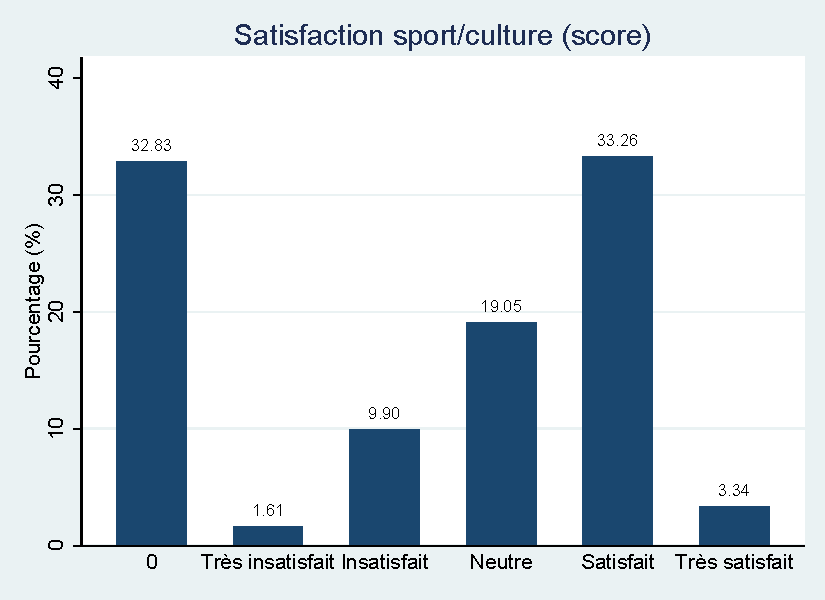
\includegraphics[width=0.6\textwidth]{../output/figures/Question_4/bar_soc_s_sportcult.pdf}
			\caption{Satisfaction par rapport aux services sportifs et culturels}
			\label{fig:bar_sport_culture}
		
	\end{figure}
		\vspace{-6pt}
		Le service sportif et culturel est celui qui tire le
		mieux son \'epingle du jeu dans la section sociale.
		\textbf{$36{,}6\%$} des \'etudiants s'en d\'eclarent
		satisfaits ou tr\`es satisfaits, contre seulement
		$11{,}5\%$ d'insatisfaits. Un tiers ($32{,}8\%$)
		dit ne pas y avoir acc\`es, et $19\%$ restent neutres.
		C'est modeste, mais c'est le meilleur score social
		de l'enqu\^ete.
		
		\begin{boiteAlerte}[Signal d'alerte]
			Avec $36{,}6\%$ de satisfaits et un score moyen de
		$2{,}28/5$, les activit\'es sportives et culturelles
		sont les \textbf{services sociaux les mieux per\c{c}us}
		de l'\'etude. Un relatif point positif dans un tableau
		global peu flatteur. 
		\end{boiteAlerte}
		
		\subsubsection{Analyse des affirmations sp\'ecifiques}
		
	
	\begin{figure}[H]
		\centering
		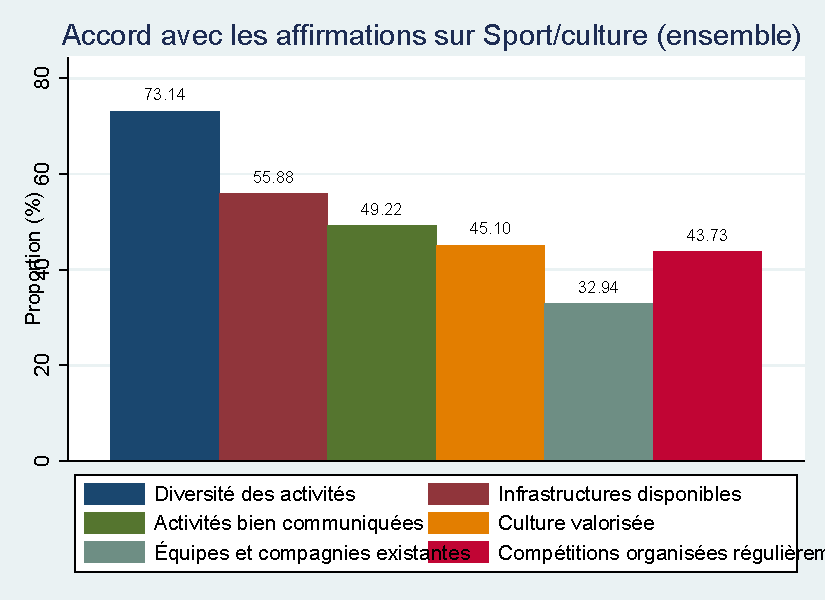
\includegraphics[width=0.6\textwidth]{../output/figures/Question_4/bar_soc_p_sportcult.pdf}
		\caption{Proportion d'accord avec les affirmations sur les services sportifs et culturels }
		\label{fig:bar_sport_cultur}
	\end{figure}
		\vspace{-6pt}
		Le point fort est indiscutable~: \textbf{7 \'etudiants sur 10}
		($73{,}1\%$) reconnaissent la \textbf{diversit\'e des activit\'es}
		propos\'ees \`a l'UNB, ce qui t\'emoigne d'une offre vari\'ee.
		Les \textbf{infrastructures} sont \'egalement jug\'ees disponibles
		par $55{,}9\%$ des r\'epondants.
		L\`a o\`u le b\^at blesse, c'est sur la \textbf{visibilit\'e
			et l'organisation}. Seulement $49{,}2\%$ estiment que les
		activit\'es sont bien communiqu\'ees --- autrement dit, la moiti\'e
		des \'etudiants n'est pas inform\'ee de ce qui se passe sur le campus.
		La \textbf{culture} est jug\'ee valoris\'ee par $45{,}1\%$ seulement,
		et l'existence d'\textbf{\'equipes et de compagnies} n'est reconnue
		que par $\mathbf{32{,}9\%}$ --- ce qui sugg\`ere que ces structures
		existent peut-\^etre, mais qu'elles ne sont pas suffisamment visibles
		ni accessibles aux yeux des \'etudiants ordinaires.Juste $43{,}73\%$ des étudiants affichent une satisfaction par rapport à l'organisation régulière des compétitions au sein de l'UNB.
		
		\begin{boiteResultat}[Bilan des services sociaux]
			\begin{itemize}[itemsep=4pt]
				\item \textbf{Meilleur service}~: sport et culture
				\textbf{$36{,}6\%$} de satisfaction.
				\item \textbf{Service le plus critiqu\'e}~: le logement avec seulement \textbf{$9{,}8\%$} d'étudiants satisfaits. --- 9 \'etudiants sur 10 sont insatisfaits.
				\item \textbf{Probl\`eme transversal}~: service de la restauration, celui de la santé cumulent des scores de satisfaction très bas, ce qui
				t\'emoigne d'une pr\'ecarit\'e sociale r\'eelle au sein de l'UNB.
			\end{itemize}
		\end{boiteResultat}
		
		
		\subsection{Satisfaction des services sociaux par rapport
			aux \'etablissements d'\'etudes}
		
		Cette partie a pour objectif de v\'erifier si la satisfaction
		des services sociaux varie d'un \'etablissement \`a un autre.
		Un score social a \'et\'e construit \`a partir des quatre
		dimensions \'evalu\'ees~: logement, sant\'e, restauration et
		activit\'es sportives et culturelles. La figure ci-dessous présente les boîtes à moustaches construits en fonction des établissements d'études.
		
			\begin{figure}[H]
			\centering
			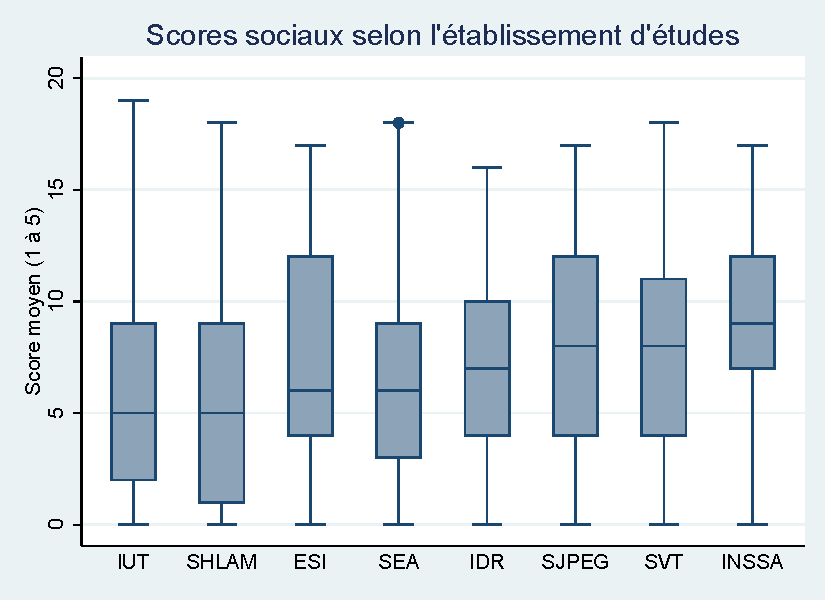
\includegraphics[width=0.6\textwidth]{../output/figures/Question_4/box_score_soc_etb.pdf}
			\caption{Satisfaction des services sociaux par rapport
				aux \'etablissements d'\'etudes}
			\label{fig:box_social_etb}
		\end{figure}
		\vspace{-6pt}
		
		La lecture des bo\^ites \`a moustaches r\'ev\`ele d'embl\'ee
		des niveaux de satisfaction in\'egaux selon les \'etablissements.
		Le \textbf{INSSA} se d\'etache avec la m\'ediane la plus
		\'elev\'ee , suivi de pr\`es par
		l'\textbf{SVT}, t\'emoignant d'une
		satisfaction sociale globalement plus marqu\'ee dans ces deux
		structures. \`A l'oppos\'e, l'\textbf{IUT} 
		et le \textbf{SHLAM}  affichent les m\'edianes
		les plus basses --- leurs \'etudiants sont, en majorit\'e, les
		moins satisfaits des services sociaux---. Il est n\'eanmoins
		important de souligner qu'\textbf{aucun \'etablissement}
		n'atteint le score neutre de $15$, signe que
		l'insatisfaction sociale est g\'en\'eralis\'ee \`a l'ensemble
		du campus.
		
		La taille g\'en\'eralement grande des bo\^ites confirme
		une \textbf{forte dispersion des avis} au sein de chaque
		\'etablissement~: les \'etudiants d'un m\^eme UFR ne partagent
		pas n\'ecessairement la m\^eme perception des services sociaux,
		ce qui sugg\`ere que d'autres facteurs jouent
		\'egalement un r\^ole.
		
		L'analyse visuelle de ces diff\'erences est-elle statistiquement
		significative~? Pour r\'epondre \`a cette question, un
		\textbf{test de Kruskal-Wallis} a \'et\'e appliqu\'e. Le test
		conclut \`a une \textbf{diff\'erence significative} entre les
		\'etablissements ( $p = 0{,}001$). Autrement
		dit, l'\'etablissement d'appartenance influence bel et bien
		la satisfaction sociale de l'\'etudiant.
		
		Des tests post-hoc de Mann-Whitney ont ensuite permis de
		localiser les \'ecarts. Afin de pr\'eserver la puissance
		statistique, les comparaisons ont \'et\'e cibl\'ees sur les
		\textbf{8~paires} opposant le Top~1 (INSSA) et
		Flop~1 (IDR)  aux autres établissements, avec un seuil de Bonferroni corrig\'e de $\alpha = 0{,}05/8 = 0{,}00625$.
		
	\vspace{-6pt}
	L'analyse de ces r\'esultats d\'esigne \textbf{IUT}
	 comme l'\'etablissement dont les \'etudiants sont les
	 moins satisfaits des services sociaux~: quatre
	 comparaisons sur huit l'impliquent comme le groupe
	 le moins bien not\'e. \`A l'inverse, \textbf{INSSA} se
	 d\'emarque positivement dans toutes les paires o\`u
	 il appara\'\i t.
	 
		\subsection{Satisfaction des services sociaux selon le sexe}
		
		Nous analyserons le niveau de satisfaction sociaux selon la répartition des étudiants en fonction de leur sexe. Pour cela, des boîtes à moustaches ont été construits. 
		\begin{figure}[H]
			\centering
			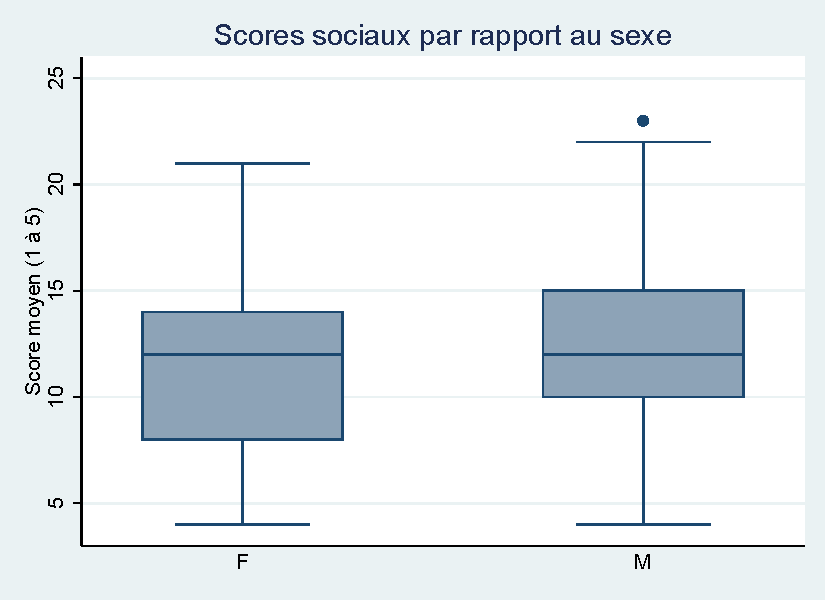
\includegraphics[width=0.6\textwidth]{../output/figures/Question_4/box_score_sociaux_sexe.pdf}
			\caption{Satisfaction des services sociaux selon le sexe}
			\label{fig:soc_sexe}
		\end{figure}
		\vspace{-6pt}
		L'analyse des bo\^ites \`a moustaches selon le sexe r\'ev\`ele
		des profils de satisfaction distincts. Les \textbf{hommes}
		affichent une m\'ediane et un positionnement g\'en\'eral de
		la bo\^ite plus \'elev\'es que ceux des \textbf{femmes},
		ce qui indique qu'ils sont globalement plus satisfaits des
		services sociaux. Cependant, cette satisfaction est loin
		d'\^etre unanime~: la partie sup\'erieure de leur bo\^ite
		--- correspondant aux \textbf{50\% des r\'epondants au-dessus
			de la m\'ediane} --- est plus \'etendue, t\'emoignant d'une
		\textbf{h\'et\'erog\'en\'eit\'e des avis} parmi les plus
		satisfaits.
		Chez les \textbf{femmes}, le sch\'ema est inverse~: c'est
		la partie \textbf{inf\'erieure} de la bo\^ite qui est plus
		dispers\'ee, ce qui signifie que les avis divergent
		principalement parmi les moins satisfaites. Les femmes ayant
		attribu\'e une note sup\'erieure \`a la m\'ediane ont en
		revanche des avis beaucoup plus homog\`enes. Ce profil
		sugg\`ere que si une partie des femmes est satisfaite de
		fa\c{c}on convergente, une autre partie exprime une
		insatisfaction vari\'ee et plus prononc\'ee.
		
		
			\section{SATISFACTION PAR RAPPORT AUX INFRASTRUCTURES ET ÉQUIPEMENTS}
		\label{sec:satisfaction par rapport aux infrastructures et équipements }
		
		L'évaluation du niveau de satisfaction des étudiants par rapport aux infrastructures et équipements passe par une analyse minutieuse des éléments de satisfaction ayant trait à la disponibilité d'internet, aux équipements mobiliers, aux équipements informatiques et aux infrastructures immobilières. Le graphique ci-dessous présente les scores de satisfaction moyens des répondants concernant ces quatre types d'infrastructures et équipements.
		
		\begin{figure}[h]
			\begin{center}
				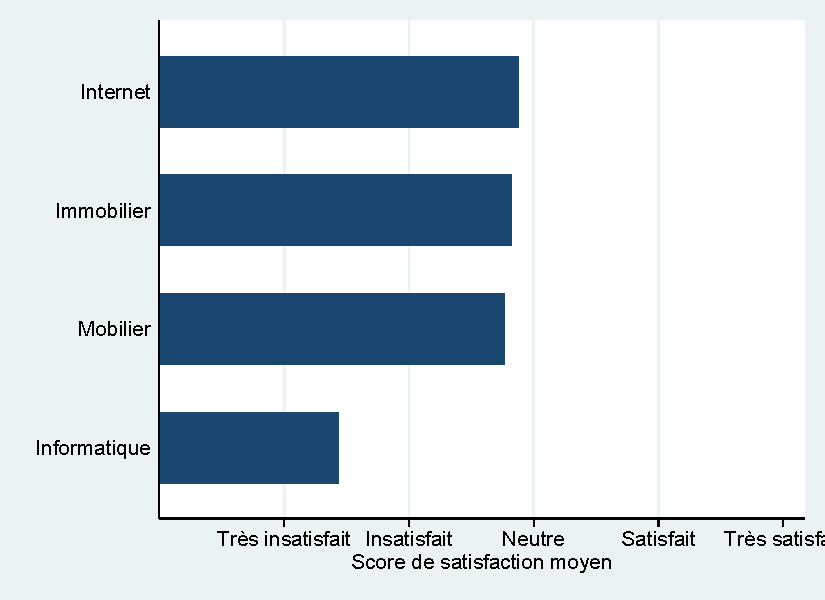
\includegraphics[scale=0.6]{../output/figures/Question_5/bar_Comparaison.pdf}
				\caption{Satisfaction par rapport aux infrastructures et équipements}
			\end{center}
		\end{figure}
		
		Une lecture d'ensemble révèle des disparités plus ou moins marquées entre les catégories. En effet, l'internet se distingue comme l'infrastructure la mieux notée, tandis que la dotation en équipements informatiques enregistre le score le plus faible, traduisant un mécontentement plus marqué sur ce point. Le mobilier et l'immobilier occupent quant à eux une position intermédiaire, avec des niveaux de satisfaction relativement proches. Afin de mieux comprendre ces écarts, passons à une analyse détaillée de chacune de ces catégories.
		
		
		\subsection{Disponibilité d'Internet à l'UNB}
		\subsubsection{Distribution des réponses et taux de satisfaction}
		La satisfaction des étudiants par rapport au volet Internet est mitigée, comme le montre le graphique ci-dessous.
		
		\begin{figure}[h]
			\begin{center}
				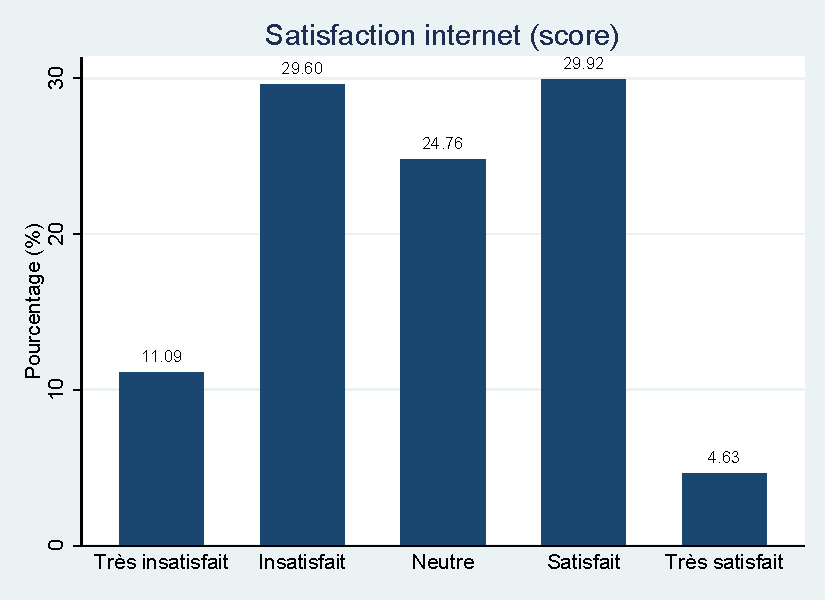
\includegraphics[scale=0.6]{../output/figures/Question_5/bar_inf_s_internet.pdf}
				\caption{Satisfaction par rapport à la disponibilité d'Internet à l'UNB}
			\end{center}
		\end{figure}
		
		En effet, les positions d'insatisfaction et de satisfaction se répartissent de manière quasi symétrique, avec respectivement 40,69\,\% de répondants insatisfaits ou très insatisfaits, contre 34,55\,\% de satisfaits ou très satisfaits. La modalité \og{}Neutre\fg{} rassemble quant à elle près d'un quart (24,8\,\%) des voix.
		Cependant, il faut souligner que l'insatisfaction domine légèrement la satisfaction, ce qui est principalement dû à la modalité \og{}Très insatisfait\fg{} qui représente à elle seule 11,09\,\% des réponses, à l'opposé des répondants \og{}Très satisfaits\fg{} qui ne cumulent que 4,63\,\% de l'échantillon, ce qui constitue d'ailleurs la proportion la plus faible de toutes les modalités.
		Ces résultats suggèrent donc que la qualité de la connexion Internet est perçue comme insuffisante par une majorité de répondants.
		\begin{table}[htbp]\centering
\def\sym#1{\ifmmode^{#1}\else\(^{#1}\)\fi}
\caption{Satisfaction internet (score)}
\begin{tabular}{l*{2}{r}}
\toprule
            &    Effectif&Fréquence (\%)\\
\midrule
Très insatisfait&         103&        11.1\\
Insatisfait &         275&        29.6\\
Neutre      &         230&        24.8\\
Satisfait   &         278&        29.9\\
Très satisfait&          43&         4.6\\
Total       &         929&       100.0\\
\bottomrule
\multicolumn{3}{l}{\footnotesize Source : Enquête, 2024. N = 929}\\
\end{tabular}
\end{table}

		
		\subsubsection{Taux d'accord avec les affirmations sur Internet}
		L'analyse des réponses relatives aux affirmations sur Internet a donné les résultats ci-dessous.
		
		\begin{figure}[!h]
			\begin{center}
				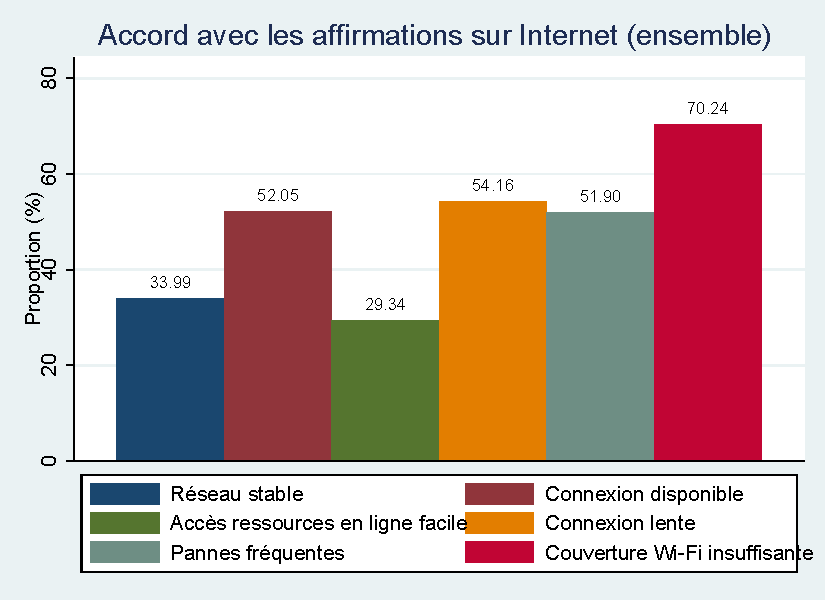
\includegraphics[scale=0.6]{../output/figures/Question_5/bar_inf_p_internet.pdf}
				\caption{Accord avec les affirmations sur Internet}
			\end{center}
		\end{figure}
		
		Le graphique révèle des résultats nuancés : une majorité d'usagers dispose d'une connexion (52,05\,\%) et 33,99\,\% jugent le réseau stable, mais plus de la moitié signale simultanément des pannes fréquentes (51,9\,\%) et 70,24\,\% estiment que la couverture Wi-Fi reste insuffisante.
		
		\paragraph{Analyse détaillée :}
		\begin{itemize}
			\item \textbf{Couverture Wi-Fi :} C'est l'indicateur qui recueille le plus de voix. En effet, sept répondants sur dix (70,24\,\%) jugent la couverture Wi-Fi insuffisante. Cette note surpasse toutes les autres et constitue de ce fait la cause majeure de l'insatisfaction dans le volet Internet.
			\item \textbf{Disponibilité de la connexion vs fréquence des pannes :} Les scores \og{}connexion disponible\fg{} (52,05\,\%) et \og{}pannes fréquentes\fg{} (51,90\,\%) sont quasi identiques. Cela indique que disponibilité ne rime pas avec fiabilité : une connexion existe mais elle reste instable.
			\item \textbf{Accès aux ressources en ligne :} Seulement un tiers des répondants (29,34\,\%) trouve l'accès aux ressources en ligne facile. Ce faible score suggère des obstacles au-delà de la simple disponibilité de la connexion.
			\item \textbf{Lenteur de la connexion et stabilité du réseau :} Le problème de la lenteur est reconnu par la majorité des répondants (54,16\,\% des voix). À cela s'ajoute le faible score de 33,99\,\% attribué à la stabilité du réseau, ce qui pourrait expliquer par ricochet les difficultés d'accès aux ressources en ligne.
		\end{itemize}
		
		
		
		\subsection{Infrastructures immobilières}
		\subsubsection{Distribution des réponses et taux de satisfaction}
		
		\begin{figure}[h]
			\begin{center}
				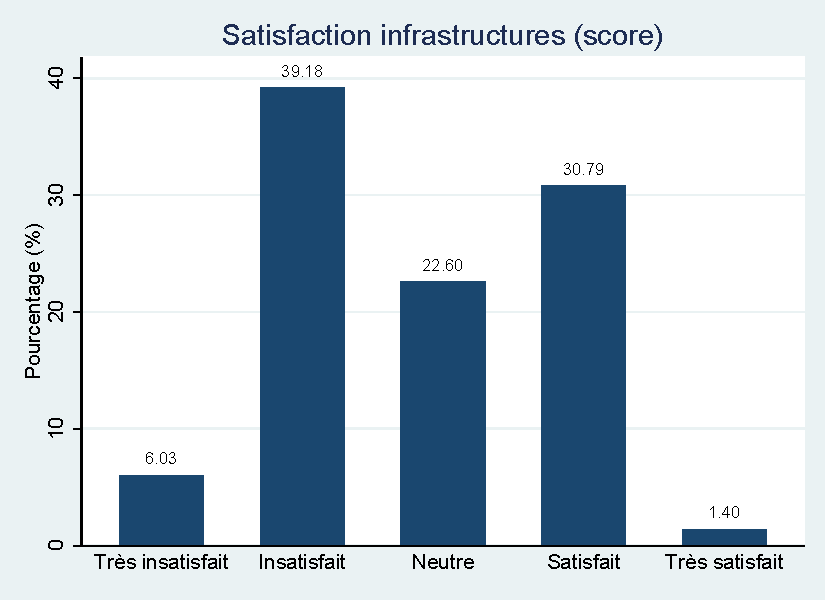
\includegraphics[scale=0.6]{../output/figures/Question_5/bar_inf_s_immobilier.pdf}
				\caption{Satisfaction par rapport aux infrastructures immobilières}
			\end{center}
		\end{figure}
		
		La distribution de la satisfaction concernant les infrastructures immobilières révèle une tendance majoritairement négative, bien qu'il y ait une proportion non négligeable de répondants satisfaits.
		En effet, l'insatisfaction constitue le point dominant, avec 45,21\,\% des répondants se déclarant insatisfaits ou très insatisfaits. La modalité \og{}Insatisfait\fg{} est particulièrement marquée, représentant à elle seule 39,18\,\% des réponses, ce qui en fait la modalité la plus fréquente de la distribution.
		À l'opposé, seuls 32,19\,\% des répondants expriment une satisfaction, dont une proportion infime de très satisfaits (1,4\,\%), laissant apparaître une appréciation très limitée de ces infrastructures. La modalité \og{}Neutre\fg{} rassemble quant à elle 22,6\,\% des répondants.
		
		\subsubsection{Taux d'accord avec les affirmations sur les infrastructures immobilières}
		L'analyse des réponses relatives aux affirmations sur les infrastructures immobilières a donné les résultats ci-après. 
		
		\begin{figure}[!h]
			\begin{center}
				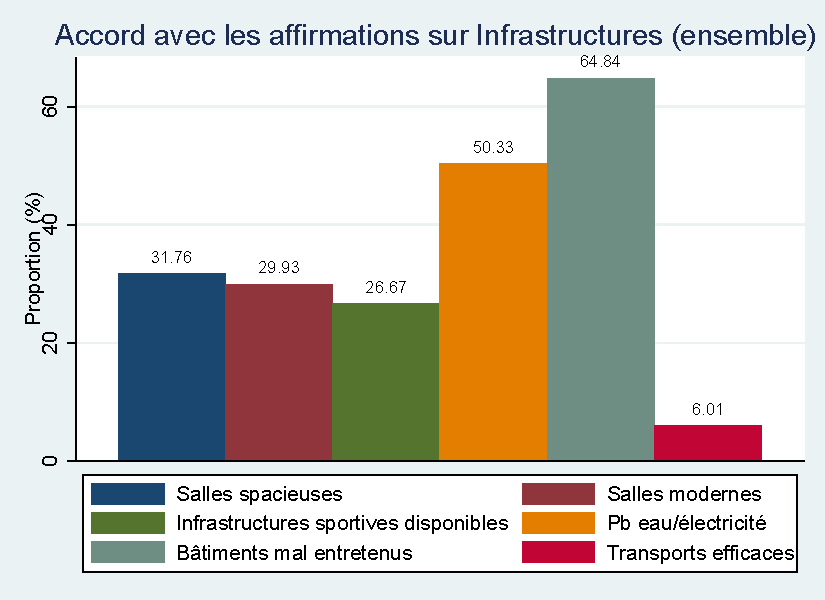
\includegraphics[scale=0.6]{../output/figures/Question_5/bar_inf_p_immobilier.pdf}
				\caption{Accord avec les affirmations sur les infrastructures immobilières}
			\end{center}
		\end{figure}
		
		Les infrastructures souffrent de problèmes sérieux : un mauvais entretien des bâtiments et la récurrence des pannes d'eau ou d'électricité (signalés respectivement par des taux alarmants de 64,84\,\% et 50,33\,\% des étudiants), ainsi qu'un problème de mobilité quasi total, avec seulement 6,01\,\% de répondants satisfaits des transports. À l'inverse, aucune affirmation positive ne dépasse le tiers des répondants.
		
		\paragraph{Analyse détaillée :}
		\begin{itemize}
			\item \textbf{Entretien des bâtiments :} Environ 65\,\% des répondants s'accordent sur le mauvais entretien des bâtiments. Ce score alarmant, qui est d'ailleurs le plus élevé de toute la distribution, reflète une perception de désintérêt.
			\item \textbf{Pannes eau/électricité :} La moitié des répondants signale des problèmes d'eau ou d'électricité. Ces défaillances aggravent directement les conditions de travail et viennent confirmer les problèmes d'entretien des bâtiments.
			\item \textbf{Transports :} Avec seulement 6,01\,\% d'accord sur l'efficacité des transports, c'est le score le plus bas du graphique. Le volet transport est donc un point critique à revoir.
			\item \textbf{Équipements :} Les salles spacieuses (31,76\,\%), modernes (29,93\,\%) et les infrastructures sportives (26,67\,\%) constituent les seuls points positifs, mais leur faible niveau d'accord montre qu'ils ne compensent pas les défauts cités plus haut.
		\end{itemize}
		
		\subsection{Équipements mobiliers}
		\subsubsection{Distribution des réponses et taux de satisfaction}
		\begin{figure}[H]
			\begin{center}
				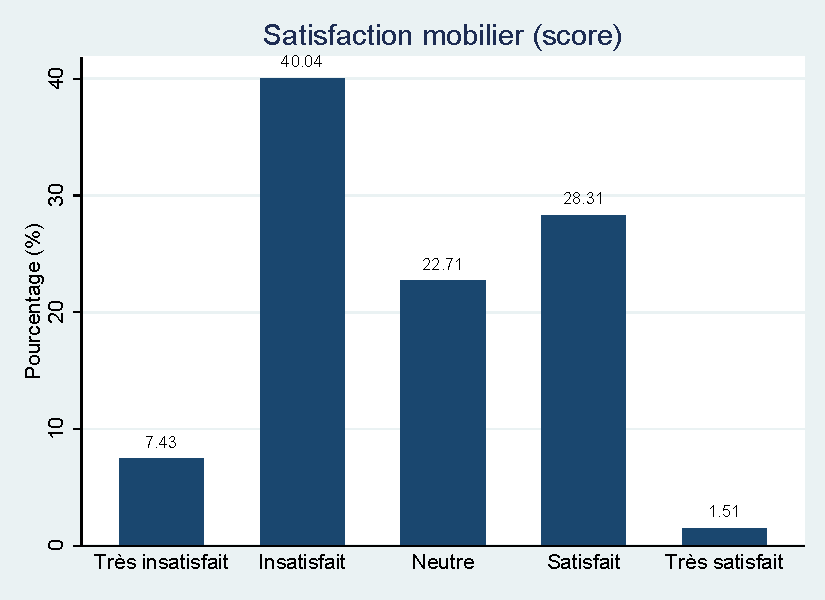
\includegraphics[scale=0.6]{../output/figures/Question_5/bar_inf_s_mobilier.pdf}
				\caption{Satisfaction par rapport aux équipements mobiliers à l'UNB}
			\end{center}
		\end{figure}
		
		La satisfaction concernant le mobilier présente une distribution similaire à celle observée au niveau de l'immobilier. En effet, \og{}Insatisfait\fg{} domine largement avec 40,04\,\% des répondants, suivi de \og{}Satisfait\fg{} (28,31\,\%) et \og{}Neutre\fg{} (22,71\,\%). En cumulant les insatisfactions, on atteint près de 47,5\,\% des répondants qui expriment un mécontentement, contre seulement 29,82\,\% de satisfaction (satisfaits + très satisfaits).
		Le taux de \og{}Très satisfaits\fg{} est particulièrement très faible (1,51\,\%). Le mobilier apparaît de ce fait comme l'un des points les plus dépréciés de l'enquête.
		
		\subsubsection{Taux d'accord avec les affirmations sur le mobilier}
		\begin{figure}[H]
			\begin{center}
				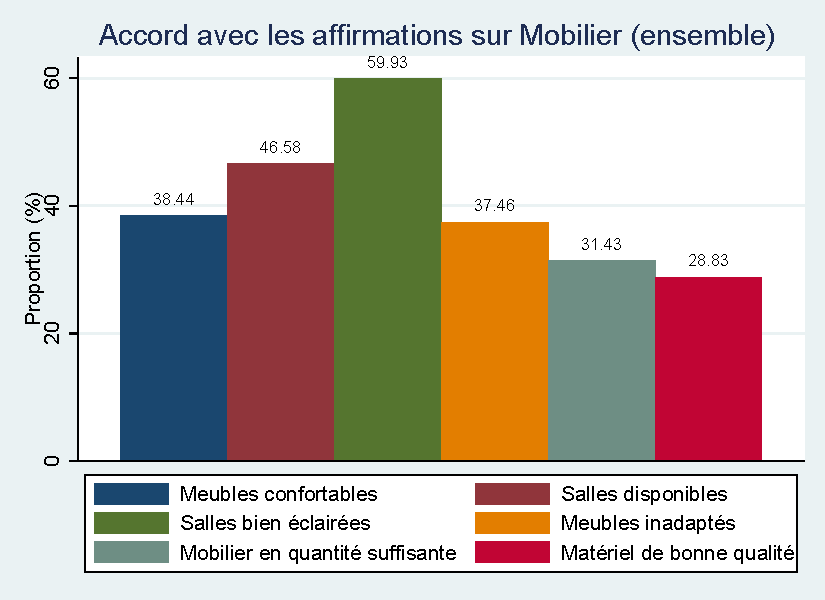
\includegraphics[scale=0.6]{../output/figures/Question_5/bar_inf_p_mobilier.pdf}
				\caption{Accord avec les affirmations sur les équipements mobiliers}
			\end{center}
		\end{figure}
		
		Le mobilier génère une contradiction flagrante : 37,46\,\% des répondants jugent les meubles inadaptés tandis que 38,44\,\% les trouvent confortables. Cette coexistence signale que certains sites sont relativement mieux équipés tandis que d'autres souffrent d'un déficit mobilier. Il faudra donc mener une analyse corrélatoire.
		
		\paragraph{Analyse détaillée :}
		\begin{itemize}
			\item \textbf{Meubles inadaptés :} Seule affirmation négative du graphique, elle concentre un score de 37,46\,\%. Cependant, l'inadaptation ne porte pas nécessairement sur l'état physique du mobilier, mais sur son inadéquation aux besoins des étudiants.
			\item \textbf{Disponibilité des salles :} Moins de la moitié des répondants (46,58\,\%) trouvent les salles disponibles. La capacité d'accueil semble donc globalement insuffisante.
			\item \textbf{Éclairage et confort :} Environ 60\,\% des répondants trouvent les salles bien éclairées. C'est d'ailleurs le score positif le plus élevé. L'éclairage semble globalement suffisant, ce qui constitue un acquis à préserver face aux autres difficultés observées. À cela s'ajoute le confort des meubles qui obtient un score de 38,4\,\%, révélant que la dotation mobilière n'est pas appréciée à l'unanimité.
			\item \textbf{Quantité et qualité du mobilier :} Le mobilier en quantité suffisante (31,43\,\%) et le matériel de bonne qualité (28,8\,\%) affichent les scores positifs les plus faibles. Moins d'un tiers des répondants juge l'équipement satisfaisant tant au niveau de la quantité que de la qualité.
		\end{itemize}
		
		\subsection{Équipements informatiques}
		\subsubsection{Distribution des réponses et taux de satisfaction}
		\begin{figure}[h]
			\begin{center}
				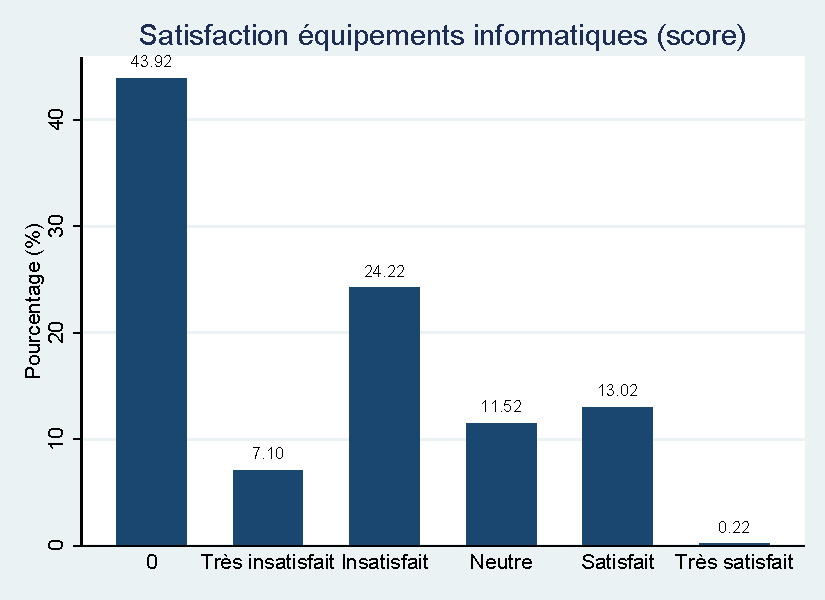
\includegraphics[scale=0.6]{../output/figures/Question_5/bar_inf_s_informatiq.pdf}
				\caption{Satisfaction par rapport aux équipements informatiques à l'UNB}
			\end{center}
		\end{figure}
		
		Avec 47,47\,\% d'insatisfaits cumulés contre seulement 29,82\,\% de satisfaits, les équipements informatiques enregistrent le pire bilan de satisfaction de la section. Le taux de très satisfaits à 1,51\,\% indique que moins d'un étudiant sur dix trouve les équipements informatiques excellents.
		
		\subsubsection{Taux d'accord avec les affirmations sur les équipements informatiques}
		\begin{figure}[h]
			\begin{center}
				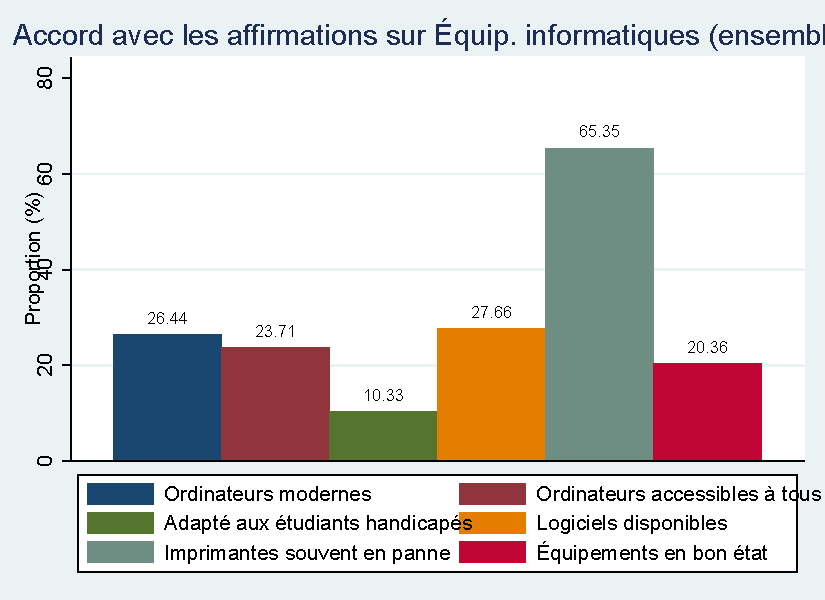
\includegraphics[scale=0.6]{../output/figures/Question_5/bar_inf_p_informatiq.pdf}
				\caption{Accord avec les affirmations sur les équipements informatiques}
			\end{center}
		\end{figure}
		
		Les analyses montrent un bilan très peu satisfaisant : 65,35\,\% signalent des pannes d'imprimantes, moins d'un quart trouve les ordinateurs modernes ou accessibles, et seulement 10,33\,\% jugent les équipements adaptés aux étudiants handicapés.
		\paragraph{Analyse détaillée :}
		\begin{itemize}
			\item \textbf{Imprimantes en panne :} C'est le score dominant du graphique, reconnu par 64,84\,\% des répondants.
			\item \textbf{Adaptation aux personnes handicapées :} Seulement un répondant sur dix juge les équipements adaptés aux besoins des personnes handicapées. Ce score alarmant met en exergue l'inadéquation des équipements informatiques à l'usage des étudiants.
			\item \textbf{Modernité et accessibilité :} Les ordinateurs modernes (26,44\,\%) et accessibles à tous (23,71\,\%) rassemblent à peine un quart des répondants. Ces scores révèlent une vétusté des équipements dont la disponibilité reste insuffisante au regard des besoins.
			\item \textbf{Bon état des équipements :} Seulement un répondant sur cinq (20,36\,\%) estime que les équipements sont en bon état. Ce score, associé aux 65,35\,\% de pannes d'imprimantes, donne une image dégradée et insuffisamment renouvelée du volet informatique.
		\end{itemize}
		
		
		
		
		
		\section{Modèle de régression logistique}
		\subsection{Description du modèle}
		L'analyse explicative de la satisfaction globale consistera à analyser les déterminants de cette dernière et à rendre compte du degré de leur influence sur la variable dépendante. La variable expliquée prend la valeur 1 ou 0 selon que l'événement étudié se réalise ou non. Dans notre échantillon de 929 étudiants d'indice $i = 1, \ldots, 929$, on observe chez chaque individu si l'événement $y$ est réalisé, $y$ étant la non-satisfaction générale. La variable $y$ étant binaire, le modèle de régression logistique convient donc et cherchera à modéliser l'alternative ($y_i = 1$ ou $y_i = 0$) et à estimer la probabilité $P_i$ associée à l'événement ($y_i = 1$).
		
		\subsection{Modèle final}
		
		\begin{table}[htbp]
\centering
\caption{Régression logistique -- Satisfaction globale des \'etudiants de l'UNB}
\label{tab:logit_sat}
\begin{tabular}{lcc}
\toprule
\textbf{Variables} & \textbf{Odds Ratio} & \textbf{p $>$ z} \\
\midrule
\multicolumn{3}{l}{\textbf{Sexe}} \\
\quad Féminin & Référece & -- \\
\quad Masculin & 0.71 & 0.019** \\
\midrule
\multicolumn{3}{l}{\textbf{Âge}} \\
\quad 19-20 & R\'ef. & -- \\
\quad 21-22 & 1.34 & 0.505NS \\
\quad 23-24 & 1.25 & 0.613NS \\
\quad 25-26 & 1.69 & 0.265NS \\
\midrule
\multicolumn{3}{l}{\textbf{Niveau d'\'etude}} \\
\quad Licence & R\'ef. & -- \\
\quad Master & 0.60 & 0.296NS \\
\quad Doctorat & 1.00 & .NS \\
\midrule
\multicolumn{3}{l}{\textbf{\'Etablissement}} \\
\quad ESI & R\'ef. & -- \\
\quad IDR & 4.34 & 0.002*** \\
\quad INSSA & 3.07 & 0.036** \\
\quad IUT & 6.01 & 0.000*** \\
\quad UFR-SEA & 4.92 & 0.001*** \\
\quad UFR-SHLAM & 7.38 & 0.000*** \\
\quad UFR-SJPEG & 4.87 & 0.001*** \\
\quad UFR-SVT & 4.14 & 0.002*** \\
\midrule
Constante & 0.21 & 0.037** \\
\midrule
\multicolumn{3}{l}{\textbf{Statistiques du mod`ele}} \\
Nombre d'observations & \multicolumn{2}{c}{891} \\
Log likelihood & \multicolumn{2}{c}{-578.38} \\
LR chi2(15) & \multicolumn{2}{c}{57.63} \\
Prob $>$ chi2 & \multicolumn{2}{c}{0.000} \\
Pseudo R\textsuperscript{2} & \multicolumn{2}{c}{0.0512} \\
\midrule
\multicolumn{3}{l}{\textbf{Test de Hosmer-Lemeshow}} \\
\quad Hosmer-Lemeshow chi2(8) & \multicolumn{2}{c}{9.56} \\
\quad Prob $>$ chi2 & \multicolumn{2}{c}{.} \\
\midrule
Aire sous la courbe ROC (AUC) & \multicolumn{2}{c}{0.6385} \\
\bottomrule
\multicolumn{3}{l}{\footnotesize \textbf{***} : significativit\'e au seuil de 1\% \quad \textbf{**} : au seuil de 5\% \quad \textbf{*} : au seuil de 10\% \quad \textbf{NS} : non significatif} \\
\multicolumn{3}{l}{\footnotesize \textit{p $>$ z} : la p-value associ\'ee au test de Wald} \\
\end{tabular}
\end{table}
		
		\subsection{Interprétation des résultats}
		\subsubsection{Validation du modèle et test de diagnostic}
		\begin{itemize}
			\item La probabilité critique associée au modèle (Prob $>$ chi2 $= 0{,}000$) est inférieure au seuil de 1\,\%, ce qui confirme que le modèle est globalement significatif. Les variables explicatives retenues contribuent conjointement à expliquer la variable dépendante.
			\item Cependant, le Pseudo $R^2$ est égal à 0,0512, ce qui signifie que les variables explicatives n'expliquent que 5,12\,\% de la variabilité de l'insatisfaction. Ce pouvoir explicatif est relativement faible, ce qui suggère que d'autres facteurs non inclus dans le modèle influencent également cette variable.
			\item L'aire sous la courbe ROC (AUC) est de 0,6385, ce qui indique une capacité discriminante acceptable mais modérée du modèle. Il distingue les satisfaits des non-satisfaits mieux qu'un classement aléatoire (AUC $= 0{,}5$).
		\end{itemize}
		
		\subsubsection{Interprétation des odds ratios}
		\paragraph{Effet du sexe :}
		L'effet du sexe est significatif au seuil de 5\,\%. Avec un odds ratio de 0,71, les étudiants de sexe masculin ont moins de chances d'être insatisfaits que les étudiantes (référence). En d'autres termes, être un homme réduit la probabilité d'être insatisfait d'environ 29\,\% par rapport aux femmes, toutes choses égales par ailleurs.
		\paragraph{Effet de l'âge :}
		Aucune modalité de la variable âge n'est statistiquement significative (toutes les p-values sont largement supérieures à 0,10). L'âge n'a donc pas d'effet significatif sur la satisfaction dans cet échantillon.
		\paragraph{Effet du niveau d'étude :}
		Les modalités Master ($OR = 0{,}60$) et Doctorat ($OR = 1{,}00$) ne sont pas significatives. Le niveau d'étude n'influence donc pas significativement la satisfaction dans ce modèle.
		\paragraph{Effet de l'établissement :}
		C'est la variable dont les effets sont les plus marqués et les plus significatifs. En prenant l'ESI comme référence, tous les autres établissements présentent des odds ratios nettement supérieurs à 1 et significatifs.
		Les étudiants de l'UFR-SHLAM ont les plus grandes chances d'être insatisfaits ($OR = 7{,}38$), suivis de l'IUT ($OR = 6{,}01$) et de l'UFR-SEA ($OR = 4{,}92$), comparativement aux étudiants de l'ESI. De manière générale, les étudiants de l'ESI sont les plus satisfaits.
		
		
		
			\chapter{Discussion}
		\label{chap:discussion}
			Ce chapitre confronte les résultats obtenus dans le cadre de la présente étude avec ceux
		issus de la littérature disponible. Il aborde successivement la satisfaction par rapport aux services administratifs, pédagogiques, sociaux,
		infrastructures et équipements, les déterminants socio-démographiques de l'insatisfaction
		globale, les limites et les forces de l'étude.
		
		\section{La satisfaction par rapport aux services administratifs}
		Les services administratifs de l'UNB pr\'esentent
		des r\'esultats in\'egaux selon les domaines.
		La s\'ecurit\'e constitue la pr\'eoccupation principale~:
		huit \'etudiants sur dix signalent des vols fr\'equents
		sur le campus ($80{,}56\,\%$), et les lacunes en
		pr\'evention sanitaire ($48{,}28\,\%$) comme en
		\'equipements de protection ($38{,}36\,\%$) alourdissent
		ce constat \citep{pascarella1991how}. La communication
		institutionnelle souffre quant \`a elle des pannes
		r\'ep\'et\'ees de Campus Faso ($63{,}96\,\%$), entra\^inant
		des informations tardives et inaccessibles pour les
		\'etudiants \citep{wiers2002student}. La d\'elivrance
		de documents reste le deuxi\`eme point faible~: plus
		de la moiti\'e des \'etudiants jugent les d\'elais non
		respect\'es, et l'absence totale de suivi num\'erique
		oblige \`a des d\'emarches r\'ep\'et\'ees \citep{elliott2002}.
		\`A l'oppos\'e, les inscriptions constituent le point
		fort de la section avec $62{,}11\,\%$ de satisfaits,
		port\'es par la num\'erisation r\'eussie du processus
		--- attestations t\'el\'echargeables, frais abordables,
		absence de d\'eplacement \citep{hill1995measuring}.
		L'accueil obtient un r\'esultat interm\'ediaire~: le
		personnel est appr\'eci\'e pour sa chaleur humaine,
		mais le suivi des dossiers reste quasi absent
		($30{,}45\,\%$) \citep{aldridge1998}.
		En somme, l'UNB doit s'appuyer sur le succ\`es de
		la num\'erisation des inscriptions pour moderniser
		ses autres proc\'edures administratives, tout en
		traitant en priorit\'e les probl\`emes de s\'ecurit\'e
		qui d\'egradent profond\'ement l'exp\'erience
		\'etudiante au quotidien.
		
		\section{La satisfaction par rapport aux services pédagogiques}
		Sur le plan p\'edagogique, les r\'esultats
		r\'ev\`elent des forces r\'eelles mais aussi
		des lacunes profondes selon les services
		\'evalu\'es. Les \'etudiants sont globalement
		satisfaits de la pertinence des fili\`eres
		($72{,}23\,\%$) et de la qualit\'e de la formation
		($70{,}83\,\%$)~: ils reconnaissent que l'UNB propose
		de bons programmes. Mais d\`es qu'on parle des
		services concrets comme les \textbf{stages} et le
		\textbf{traitement des r\'eclamations}, la situation
		change radicalement. Plus d'un \'etudiant sur deux
		d\'eclare que le service des stages n'existe tout
		simplement pas dans son \'etablissement --- ce n'est
		pas un probl\`eme de qualit\'e, c'est un probl\`eme
		d'existence \citep{marzo2005}.
		Les diff\'erences entre \'etablissements ne sont pas
		le fruit du hasard. L'\textbf{INSSA} se distingue
		positivement, tandis que \textbf{SHLAM} affiche les
		scores les plus bas. Concr\`etement, deux \'etudiants
		de l'UNB n'ont pas la m\^eme exp\'erience selon leur
		UFR --- ce qui soul\`eve une question d'\'equit\'e
		que l'administration ne peut pas ignorer
		\citep{kuh2006}.
		Enfin, les doctorants sont les plus satisfaits des
		services p\'edagogiques, ce qui n'est pas
		surprenant~: ils b\'en\'eficient d'un suivi plus
		personnalis\'e. \`A l'inverse, les \'etudiants en
		\textbf{Licence} --- qui repr\'esentent pourtant
		$82\,\%$ des effectifs --- expriment les niveaux
		d'insatisfaction les plus \'elev\'es. C'est donc
		sur eux que les efforts d'am\'elioration doivent
		se concentrer en priorit\'e.
		
		
		\section{La satisfaction par rapport aux services sociaux}
			Les services sociaux pr\'esentent le bilan le plus
		pr\'eoccupant~: aucun des quatre domaines \'evalu\'es
		n'atteint le score neutre. Le logement et la restauration
		concentrent l'essentiel de l'insatisfaction, tandis que
		les activit\'es sportives et culturelles constituent le
		seul point d'appui relatif, avec $36{,}6\,\%$ de
		satisfaits \citep{amole2009}.
		Les disparit\'es inter-\'etablissements ne sont pas
		al\'eatoires~: l'\textbf{INSSA} se distingue positivement, tandis que
		\textbf{IUT} affiche syst\'ematiquement les scores les
		plus bas.
		Concernant le sexe, les \textbf{hommes} affichent
		globalement une satisfaction sociale plus \'elev\'ee
		que les \textbf{femmes}, dont la distribution montre
		une plus forte dispersion vers le bas. Ce r\'esultat
		sugg\`ere que les femmes 
		subissent plus directement la pr\'ecarit\'e des
		conditions de vie universitaires. 
		
		
		\section{La satisfaction par rapport aux infrastructures et équipements}
		L'analyse de la satisfaction des étudiants de l'UNB révèle un bilan globalement défavorable sur l'ensemble des critères évaluées. Concernant les infrastructures et équipements, quatre domaines ont été examinés, tous affichant des taux d'insatisfaction supérieurs aux taux de satisfaction. La disponibilité d'Internet concentre les principales plaintes des étudiants, notamment la couverture Wi-Fi insuffisante (70,24 \%), la lenteur de la connexion (54,16 \%) et les pannes fréquentes (51,90 \%). Les infrastructures immobilières souffrent quant à elles d'un mauvais entretien et de coupures fréquentes d'eau et d'électricité, tandis que la qualité des équipements mobiliers est très inégale selon les sites. Les équipements informatiques enregistrent le bilan le plus alarmant, avec 47,47 \% d'insatisfaits,un matériel informatique clairement vieux et dégradé et une quasi inadéquation pour les personnes en situation de handicap.
		
		\section{Les déterminants socio-démographiques de l'insatisfaction globale}
		
		Sur le plan socio-démographique, le sexe et l'établissement de rattachement constituent les deux seuls déterminants significatifs de l'insatisfaction globale. Les étudiantes se révèlent plus exposées à l'insatisfaction que leurs homologues masculins (OR = 0,71), certainement à cause d'une offre de services moins adaptée à leurs besoins. L'âge et le niveau d'étude n'exercent aucun effet significatif. En revanche, l'établissement de rattachement s'impose comme le facteur le plus déterminant. En effet les étudiants de l'ESI affichent les niveaux de satisfaction les plus élevés, tandis que ceux de l'UFR-SHLAM (OR = 7,38) et de l'IUT (OR = 6,01) expriment la plus forte insatisfaction. Il convient donc de mener des politiques d'amélioration adaptées aux différentes réalités.
		
		\section{Limites de l'étude}
		
		La présente étude n'est pas sans limites. Premièrement, la variable dépendante du modèle
		logistique~--- l'insatisfaction globale~--- a été construite à partir d'un seuil arbitraire
		(score $\leq 45$) qui, bien que fourni dans les instructions du projet, pourrait influencer
		les résultats. Une analyse de sensibilité avec d'autres seuils aurait pu renforcer la
		robustesse des conclusions.
		
		Deuxièmement, le Pseudo~$R^2$ du modèle est faible (0,0512), signifiant que les variables
		socio-démographiques retenues n'expliquent qu'une fraction limitée de la variabilité de
		l'insatisfaction. Des variables absentes du modèle~--- telles que le lieu de résidence,
		le statut socio-économique, ou les attentes initiales de l'étudiant~--- pourraient
		contribuer significativement à l'explication de la satisfaction globale.
		
		Troisièmement, la nature transversale de l'enquête ne permet pas d'établir des relations
		de causalité entre les variables explicatives et la satisfaction. Une étude longitudinale
		permettrait de mieux saisir l'évolution de la satisfaction au fil du parcours universitaire.

		Quatrièmement,  
		dans le cadre de
		la même institution, l'absence d'une liste exhaustive et actualisée des étudiants de
		l'UNB constitue un obstacle à la mise en œuvre d'un plan de sondage probabiliste
		strictement représentatif.
		
		\section{Forces de l'étude}
		
		Malgré ces limites, l'étude présente plusieurs forces notables. Elle repose sur un
		échantillon large de 891 observations, couvrant l'ensemble des établissements de l'UNB,
		ce qui confère une bonne représentativité institutionnelle aux résultats. La combinaison
		d'une analyse descriptive détaillée et d'un modèle explicatif permet d'appréhender la
		satisfaction à la fois dans sa dimension descriptive et dans ses déterminants. Le recours
		à des indicateurs validés de qualité du modèle (Pseudo~$R^2$, test de Hosmer-Lemeshow,
		courbe ROC) garantit la rigueur de l'analyse explicative.
		
		Enfin, sur le plan pédagogique, ce travail s'inscrit dans la tradition des enquêtes
		menées par les étudiants de LSI de l'UNB et contribue à la constitution d'un corpus de données empiriques
		sur les conditions de vie étudiante à l'UNB, dont la production reste encore insuffisante
		au Burkina Faso.
		
		\chapter{CONCLUSION ET RECOMMANDATIONS}
	\section{Conclusion}
	
	Cette \'etude avait pour objectif d'\'evaluer la
	satisfaction des \'etudiants de l'Universit\'e Nazi
	Boni vis-\`a-vis des services universitaires, \`a
	partir d'une enqu\^ete men\'ee aupr\`es de $929$
	\'etudiants r\'epartis dans huit \'etablissements.
	Les r\'esultats sont clairs~: la satisfaction n'est
	pas uniforme. Les \'etudiants reconnaissent la
	qualit\'e de leurs enseignants ($85{,}05\,\%$) et la
	diversit\'e des fili\`eres propos\'ees ($81{,}19\,\%$).
	Mais d\`es qu'on touche aux services concrets ---
	logement, restauration, stages, s\'ecurit\'e,
	gestion documentaire --- le tableau se d\'egrade.
	Le service des stages reste inaccessible pour plus
	d'un \'etudiant sur deux malgr\'e l'existence des
	bureaux d\'edi\'es, et les infrastructures
	num\'eriques souffrent de pannes r\'ecurrentes qui
	perturbent le quotidien acad\'emique.
	La r\'egression logistique a permis d'identifier
	les deux seuls d\'eterminants significatifs de
	l'insatisfaction globale~: le \textbf{sexe} et
	l'\textbf{\'etablissement de rattachement}. Les
	\'etudiantes sont plus expos\'ees \`a l'insatisfaction
	($OR = 0{,}6385$), et les \'etudiants du \textbf{SHLAM}
	($OR = 7{,}38$) et de l'\textbf{IUT} ($OR = 6{,}01$)
	sont ceux qui souffrent le plus --- tandis que
	l'\textbf{ESI} se d\'etache comme l'\'etablissement
	le plus satisfaisant.
	
	
	\section{Récommandations}
	Sur la base de ces r\'esultats, nous formulons
	cinq recommandations \`a l'intention de
	l'administration de l'UNB~:
	
	\begin{enumerate}[label=\textbf{R\arabic*.},
		leftmargin=2.5em]
		
		\item \textbf{Am\'eliorer les prestations des
			bureaux de stages existants}~: bien que ces
		structures soient d\'ej\`a en place, plus d'un
		\'etudiant sur deux d\'eclare que le service
		des stages est inaccessible dans son
		\'etablissement. Il est donc urgent de renforcer
		leur visibilit\'e, d'\'elargir leur portefeuille
		de partenaires entreprises, de formaliser le
		suivi des \'etudiants en stage et de garantir
		une offre \'equitable entre tous les
		\'etablissements. Un bureau qui existe mais
		que les \'etudiants ne connaissent pas ou ne
		peuvent pas utiliser, c'est comme s'il
		n'existait pas.
		\item \textbf{S\'ecuriser le campus en urgence}
		en installant des syst\`emes de surveillance,
		en renfor\c{c}ant la pr\'esence du personnel
		de s\'ecurit\'e et en mettant en place des
		dispositifs de pr\'evention du vol. Un
		\'etudiant qui craint pour ses affaires ne
		peut pas se concentrer sur ses \'etudes.
		\item \textbf{Am\'eliorer la connectivit\'e
			Internet} sur l'ensemble des sites, en
		comblant les zones sans couverture Wi-Fi et
		en r\'eduisant les pannes fr\'equentes qui
		paralysent la plateforme Campus Faso.
		\item \textbf{Adopter une politique
			d'am\'elioration cibl\'ee} par \'etablissement,
		en allouant prioritairement les ressources
		aux structures les plus en difficult\'e~:
		SHLAM et IUT en premier lieu, o\`u les
		niveaux d'insatisfaction sont les plus
		alarm\'ants.
		\item \textbf{Mieux prendre en compte les
			besoins sp\'ecifiques des \'etudiantes}, dont
		le niveau d'insatisfaction syst\'ematiquement
		plus \'elev\'e --- notamment sur le logement
		et la restauration --- appelle des r\'eponses
		institutionnelles concr\`etes et adapt\'ees.
		
	\end{enumerate}
	
	
		
		
% ============================================================
%  BIBLIOGRAPHIE
% ============================================================
\cleardoublepage
\addcontentsline{toc}{chapter}{BIBLIOGRAPHIE}
\nocite{*}
\bibliographystyle{apalike}   % style auteur-date (Harvard)
\bibliography{references}     % nom de ton fichier .bib
% ============================================================
%  ANNEXES
% ============================================================
\addcontentsline{toc}{chapter}{ANNEXES}
\appendix
\cleardoublepage


\chapter{}
\label{ann:resume}
\begin{table}[H]
	\centering
	\caption{Classement des services les mieux évalués et ceux les critiqués}
	\label{tab:coefficients}
	
	\begin{tabular}{clcc}
		\toprule
		\rowcolor{couleurPrimaire!20}
		\textbf{Rang} & \textbf{Service / Affirmation} & \textbf{\% Oui} & \textbf{\% Non} \\
		\midrule
		1 & Enseignants expérimentés & 85 & 15 \\
		2 & Diversité des filières & 81.19 & 18.8 \\
		107 & Adapté aux étudiants handicapés & 10.3 & 89.7 \\
		108 & Transports efficaces & 6 & 94 \\
		\bottomrule
	\end{tabular}
	
\end{table}

		
		
\end{document}